\documentclass[twoside]{book}

% Packages required by doxygen
\usepackage{fixltx2e}
\usepackage{calc}
\usepackage{doxygen}
\usepackage[export]{adjustbox} % also loads graphicx
\usepackage{graphicx}
\usepackage[utf8]{inputenc}
\usepackage{makeidx}
\usepackage{multicol}
\usepackage{multirow}
\PassOptionsToPackage{warn}{textcomp}
\usepackage{textcomp}
\usepackage[nointegrals]{wasysym}
\usepackage[table]{xcolor}

% Font selection
\usepackage[T1]{fontenc}
\usepackage[scaled=.90]{helvet}
\usepackage{courier}
\usepackage{amssymb}
\usepackage{sectsty}
\renewcommand{\familydefault}{\sfdefault}
\allsectionsfont{%
  \fontseries{bc}\selectfont%
  \color{darkgray}%
}
\renewcommand{\DoxyLabelFont}{%
  \fontseries{bc}\selectfont%
  \color{darkgray}%
}
\newcommand{\+}{\discretionary{\mbox{\scriptsize$\hookleftarrow$}}{}{}}

% Page & text layout
\usepackage{geometry}
\geometry{%
  a4paper,%
  top=2.5cm,%
  bottom=2.5cm,%
  left=2.5cm,%
  right=2.5cm%
}
\tolerance=750
\hfuzz=15pt
\hbadness=750
\setlength{\emergencystretch}{15pt}
\setlength{\parindent}{0cm}
\setlength{\parskip}{3ex plus 2ex minus 2ex}
\makeatletter
\renewcommand{\paragraph}{%
  \@startsection{paragraph}{4}{0ex}{-1.0ex}{1.0ex}{%
    \normalfont\normalsize\bfseries\SS@parafont%
  }%
}
\renewcommand{\subparagraph}{%
  \@startsection{subparagraph}{5}{0ex}{-1.0ex}{1.0ex}{%
    \normalfont\normalsize\bfseries\SS@subparafont%
  }%
}
\makeatother

% Headers & footers
\usepackage{fancyhdr}
\pagestyle{fancyplain}
\fancyhead[LE]{\fancyplain{}{\bfseries\thepage}}
\fancyhead[CE]{\fancyplain{}{}}
\fancyhead[RE]{\fancyplain{}{\bfseries\leftmark}}
\fancyhead[LO]{\fancyplain{}{\bfseries\rightmark}}
\fancyhead[CO]{\fancyplain{}{}}
\fancyhead[RO]{\fancyplain{}{\bfseries\thepage}}
\fancyfoot[LE]{\fancyplain{}{}}
\fancyfoot[CE]{\fancyplain{}{}}
\fancyfoot[RE]{\fancyplain{}{\bfseries\scriptsize Generated by Doxygen }}
\fancyfoot[LO]{\fancyplain{}{\bfseries\scriptsize Generated by Doxygen }}
\fancyfoot[CO]{\fancyplain{}{}}
\fancyfoot[RO]{\fancyplain{}{}}
\renewcommand{\footrulewidth}{0.4pt}
\renewcommand{\chaptermark}[1]{%
  \markboth{#1}{}%
}
\renewcommand{\sectionmark}[1]{%
  \markright{\thesection\ #1}%
}

% Indices & bibliography
\usepackage{natbib}
\usepackage[titles]{tocloft}
\setcounter{tocdepth}{3}
\setcounter{secnumdepth}{5}
\makeindex

% Hyperlinks (required, but should be loaded last)
\usepackage{ifpdf}
\ifpdf
  \usepackage[pdftex,pagebackref=true]{hyperref}
\else
  \usepackage[ps2pdf,pagebackref=true]{hyperref}
\fi
\hypersetup{%
  colorlinks=true,%
  linkcolor=blue,%
  citecolor=blue,%
  unicode%
}

% Custom commands
\newcommand{\clearemptydoublepage}{%
  \newpage{\pagestyle{empty}\cleardoublepage}%
}

\usepackage{caption}
\captionsetup{labelsep=space,justification=centering,font={bf},singlelinecheck=off,skip=4pt,position=top}

%===== C O N T E N T S =====

\begin{document}

% Titlepage & ToC
\hypersetup{pageanchor=false,
             bookmarksnumbered=true,
             pdfencoding=unicode
            }
\pagenumbering{alph}
\begin{titlepage}
\vspace*{7cm}
\begin{center}%
{\Large Rapid\+Lib \\[1ex]\large v0.\+1.\+2 }\\
\vspace*{1cm}
{\large Generated by Doxygen 1.8.13}\\
\end{center}
\end{titlepage}
\clearemptydoublepage
\pagenumbering{roman}
\tableofcontents
\clearemptydoublepage
\pagenumbering{arabic}
\hypersetup{pageanchor=true}

%--- Begin generated contents ---
\chapter{Hierarchical Index}
\section{Class Hierarchy}
This inheritance list is sorted roughly, but not completely, alphabetically\+:\begin{DoxyCompactList}
\item \contentsline{section}{base\+Model}{\pageref{classbase_model}}{}
\begin{DoxyCompactList}
\item \contentsline{section}{knn\+Classification}{\pageref{classknn_classification}}{}
\item \contentsline{section}{neural\+Network}{\pageref{classneural_network}}{}
\end{DoxyCompactList}
\item \contentsline{section}{model\+Set}{\pageref{classmodel_set}}{}
\begin{DoxyCompactList}
\item \contentsline{section}{classification}{\pageref{classclassification}}{}
\item \contentsline{section}{regression}{\pageref{classregression}}{}
\end{DoxyCompactList}
\item \contentsline{section}{training\+Example}{\pageref{structtraining_example}}{}
\end{DoxyCompactList}

\chapter{Class Index}
\section{Class List}
Here are the classes, structs, unions and interfaces with brief descriptions\+:\begin{DoxyCompactList}
\item\contentsline{section}{\hyperlink{classbase_model}{base\+Model} }{\pageref{classbase_model}}{}
\item\contentsline{section}{\hyperlink{classclassification}{classification} }{\pageref{classclassification}}{}
\item\contentsline{section}{\hyperlink{classknn_classification}{knn\+Classification} }{\pageref{classknn_classification}}{}
\item\contentsline{section}{\hyperlink{classmodel_set}{model\+Set} }{\pageref{classmodel_set}}{}
\item\contentsline{section}{\hyperlink{classneural_network}{neural\+Network} }{\pageref{classneural_network}}{}
\item\contentsline{section}{\hyperlink{classregression}{regression} }{\pageref{classregression}}{}
\item\contentsline{section}{\hyperlink{structtraining_example}{training\+Example} }{\pageref{structtraining_example}}{}
\end{DoxyCompactList}

\chapter{File Index}
\section{File List}
Here is a list of all files with brief descriptions\+:\begin{DoxyCompactList}
\item\contentsline{section}{\hyperlink{base_model_8h}{base\+Model.\+h} }{\pageref{base_model_8h}}{}
\item\contentsline{section}{\hyperlink{classification_8cpp}{classification.\+cpp} }{\pageref{classification_8cpp}}{}
\item\contentsline{section}{\hyperlink{classification_8h}{classification.\+h} }{\pageref{classification_8h}}{}
\item\contentsline{section}{\hyperlink{classification_embindings_8h}{classification\+Embindings.\+h} }{\pageref{classification_embindings_8h}}{}
\item\contentsline{section}{\hyperlink{knn_classification_8cpp}{knn\+Classification.\+cpp} }{\pageref{knn_classification_8cpp}}{}
\item\contentsline{section}{\hyperlink{knn_classification_8h}{knn\+Classification.\+h} }{\pageref{knn_classification_8h}}{}
\item\contentsline{section}{\hyperlink{knn_embindings_8h}{knn\+Embindings.\+h} }{\pageref{knn_embindings_8h}}{}
\item\contentsline{section}{\hyperlink{model_set_8cpp}{model\+Set.\+cpp} }{\pageref{model_set_8cpp}}{}
\item\contentsline{section}{\hyperlink{model_set_8h}{model\+Set.\+h} }{\pageref{model_set_8h}}{}
\item\contentsline{section}{\hyperlink{model_set_embindings_8h}{model\+Set\+Embindings.\+h} }{\pageref{model_set_embindings_8h}}{}
\item\contentsline{section}{\hyperlink{neural_network_8cpp}{neural\+Network.\+cpp} }{\pageref{neural_network_8cpp}}{}
\item\contentsline{section}{\hyperlink{neural_network_8h}{neural\+Network.\+h} }{\pageref{neural_network_8h}}{}
\item\contentsline{section}{\hyperlink{nn_embindings_8h}{nn\+Embindings.\+h} }{\pageref{nn_embindings_8h}}{}
\item\contentsline{section}{\hyperlink{regression_8cpp}{regression.\+cpp} }{\pageref{regression_8cpp}}{}
\item\contentsline{section}{\hyperlink{regression_8h}{regression.\+h} }{\pageref{regression_8h}}{}
\item\contentsline{section}{\hyperlink{regression_embindings_8h}{regression\+Embindings.\+h} }{\pageref{regression_embindings_8h}}{}
\item\contentsline{section}{\hyperlink{training_example_8h}{training\+Example.\+h} }{\pageref{training_example_8h}}{}
\item\contentsline{section}{\hyperlink{training_example_embindings_8h}{training\+Example\+Embindings.\+h} }{\pageref{training_example_embindings_8h}}{}
\end{DoxyCompactList}

\chapter{Class Documentation}
\hypertarget{classbase_model}{}\section{base\+Model Class Reference}
\label{classbase_model}\index{base\+Model@{base\+Model}}


{\ttfamily \#include $<$base\+Model.\+h$>$}



Inheritance diagram for base\+Model\+:\nopagebreak
\begin{figure}[H]
\begin{center}
\leavevmode
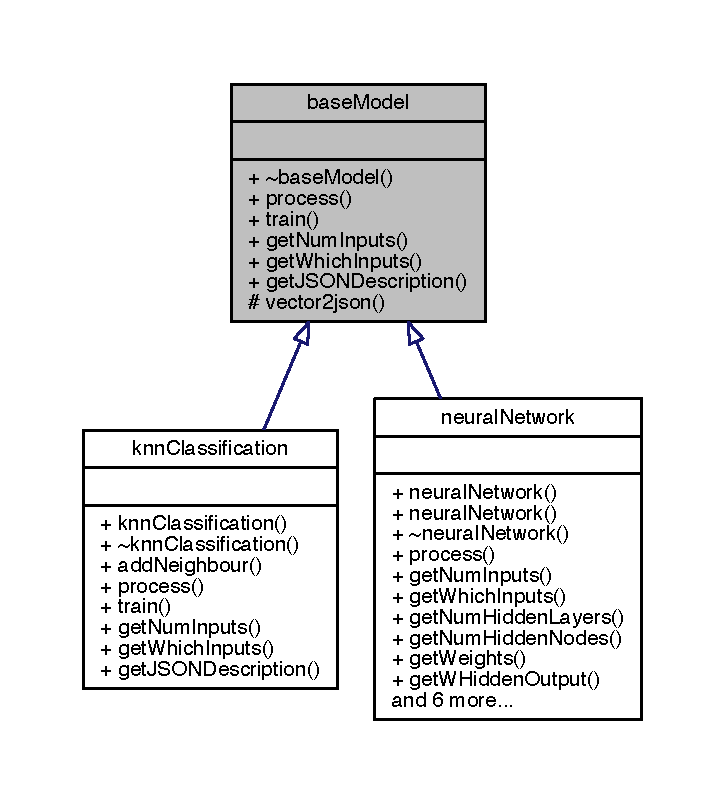
\includegraphics[width=348pt]{classbase_model__inherit__graph}
\end{center}
\end{figure}


Collaboration diagram for base\+Model\+:\nopagebreak
\begin{figure}[H]
\begin{center}
\leavevmode
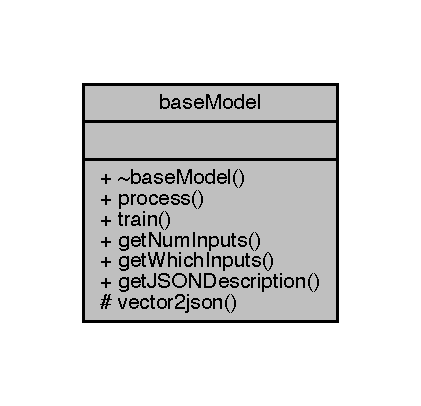
\includegraphics[width=202pt]{classbase_model__coll__graph}
\end{center}
\end{figure}
\subsection*{Public Member Functions}
\begin{DoxyCompactItemize}
\item 
virtual \hyperlink{classbase_model_a7c96328a8eda015d7f1b3d195e2fd567}{$\sim$base\+Model} ()
\item 
virtual double \hyperlink{classbase_model_a95ef1dffc2857cdd1a57c23f5f9ee2d1}{process} (const std\+::vector$<$ double $>$ \&input\+Vector)=0
\item 
virtual void \hyperlink{classbase_model_ab6cbd549d6742029ab9768bc88467b4f}{train} (const std\+::vector$<$ \hyperlink{structtraining_example}{training\+Example} $>$ \&training\+Set)=0
\item 
virtual int \hyperlink{classbase_model_a1601088280ebe5be525fd1fe49d4b1e1}{get\+Num\+Inputs} ()=0
\item 
virtual std\+::vector$<$ int $>$ \hyperlink{classbase_model_a5d6b7579536f5713eed0b7b4a6687a16}{get\+Which\+Inputs} ()=0
\item 
virtual void \hyperlink{classbase_model_a54c7ba2132721c2f990ea2fe2313f863}{get\+J\+S\+O\+N\+Description} (Json\+::\+Value \&current\+Model)=0
\end{DoxyCompactItemize}
\subsection*{Protected Member Functions}
\begin{DoxyCompactItemize}
\item 
{\footnotesize template$<$typename T $>$ }\\Json\+::\+Value \hyperlink{classbase_model_a853d3a2d610c43fca37676ac1459e3b9}{vector2json} (T vec)
\end{DoxyCompactItemize}


\subsection{Detailed Description}
Base class for wekinator models. Implemented by NN and K\+NN classes 

\subsection{Constructor \& Destructor Documentation}
\mbox{\Hypertarget{classbase_model_a7c96328a8eda015d7f1b3d195e2fd567}\label{classbase_model_a7c96328a8eda015d7f1b3d195e2fd567}} 
\index{base\+Model@{base\+Model}!````~base\+Model@{$\sim$base\+Model}}
\index{````~base\+Model@{$\sim$base\+Model}!base\+Model@{base\+Model}}
\subsubsection{\texorpdfstring{$\sim$base\+Model()}{~baseModel()}}
{\footnotesize\ttfamily virtual base\+Model\+::$\sim$base\+Model (\begin{DoxyParamCaption}{ }\end{DoxyParamCaption})\hspace{0.3cm}{\ttfamily [inline]}, {\ttfamily [virtual]}}



\subsection{Member Function Documentation}
\mbox{\Hypertarget{classbase_model_a54c7ba2132721c2f990ea2fe2313f863}\label{classbase_model_a54c7ba2132721c2f990ea2fe2313f863}} 
\index{base\+Model@{base\+Model}!get\+J\+S\+O\+N\+Description@{get\+J\+S\+O\+N\+Description}}
\index{get\+J\+S\+O\+N\+Description@{get\+J\+S\+O\+N\+Description}!base\+Model@{base\+Model}}
\subsubsection{\texorpdfstring{get\+J\+S\+O\+N\+Description()}{getJSONDescription()}}
{\footnotesize\ttfamily virtual void base\+Model\+::get\+J\+S\+O\+N\+Description (\begin{DoxyParamCaption}\item[{Json\+::\+Value \&}]{current\+Model }\end{DoxyParamCaption})\hspace{0.3cm}{\ttfamily [pure virtual]}}



Implemented in \hyperlink{classneural_network_a83f5c57ed3f555cd534a6f4ea425dfb7}{neural\+Network}, and \hyperlink{classknn_classification_a456b4b1b0fedb8f8fbe6d810bd80ceb8}{knn\+Classification}.

\mbox{\Hypertarget{classbase_model_a1601088280ebe5be525fd1fe49d4b1e1}\label{classbase_model_a1601088280ebe5be525fd1fe49d4b1e1}} 
\index{base\+Model@{base\+Model}!get\+Num\+Inputs@{get\+Num\+Inputs}}
\index{get\+Num\+Inputs@{get\+Num\+Inputs}!base\+Model@{base\+Model}}
\subsubsection{\texorpdfstring{get\+Num\+Inputs()}{getNumInputs()}}
{\footnotesize\ttfamily virtual int base\+Model\+::get\+Num\+Inputs (\begin{DoxyParamCaption}{ }\end{DoxyParamCaption})\hspace{0.3cm}{\ttfamily [pure virtual]}}



Implemented in \hyperlink{classneural_network_aaf9ff8b1a88126fcffc1e9f07a4ffe49}{neural\+Network}, and \hyperlink{classknn_classification_a3f9c8fb78c6a66f0ab9440629140400d}{knn\+Classification}.

\mbox{\Hypertarget{classbase_model_a5d6b7579536f5713eed0b7b4a6687a16}\label{classbase_model_a5d6b7579536f5713eed0b7b4a6687a16}} 
\index{base\+Model@{base\+Model}!get\+Which\+Inputs@{get\+Which\+Inputs}}
\index{get\+Which\+Inputs@{get\+Which\+Inputs}!base\+Model@{base\+Model}}
\subsubsection{\texorpdfstring{get\+Which\+Inputs()}{getWhichInputs()}}
{\footnotesize\ttfamily virtual std\+::vector$<$int$>$ base\+Model\+::get\+Which\+Inputs (\begin{DoxyParamCaption}{ }\end{DoxyParamCaption})\hspace{0.3cm}{\ttfamily [pure virtual]}}



Implemented in \hyperlink{classneural_network_afc93cb28c3897d4d1faa4ac8fbf0c1f8}{neural\+Network}, and \hyperlink{classknn_classification_af7db9297f695e67df6af08719da37921}{knn\+Classification}.

\mbox{\Hypertarget{classbase_model_a95ef1dffc2857cdd1a57c23f5f9ee2d1}\label{classbase_model_a95ef1dffc2857cdd1a57c23f5f9ee2d1}} 
\index{base\+Model@{base\+Model}!process@{process}}
\index{process@{process}!base\+Model@{base\+Model}}
\subsubsection{\texorpdfstring{process()}{process()}}
{\footnotesize\ttfamily virtual double base\+Model\+::process (\begin{DoxyParamCaption}\item[{const std\+::vector$<$ double $>$ \&}]{input\+Vector }\end{DoxyParamCaption})\hspace{0.3cm}{\ttfamily [pure virtual]}}



Implemented in \hyperlink{classneural_network_a2d93cf6790db969ea067e8588b10d204}{neural\+Network}, and \hyperlink{classknn_classification_aedeef4367ed652c768eaf5682c8ec276}{knn\+Classification}.

\mbox{\Hypertarget{classbase_model_ab6cbd549d6742029ab9768bc88467b4f}\label{classbase_model_ab6cbd549d6742029ab9768bc88467b4f}} 
\index{base\+Model@{base\+Model}!train@{train}}
\index{train@{train}!base\+Model@{base\+Model}}
\subsubsection{\texorpdfstring{train()}{train()}}
{\footnotesize\ttfamily virtual void base\+Model\+::train (\begin{DoxyParamCaption}\item[{const std\+::vector$<$ \hyperlink{structtraining_example}{training\+Example} $>$ \&}]{training\+Set }\end{DoxyParamCaption})\hspace{0.3cm}{\ttfamily [pure virtual]}}



Implemented in \hyperlink{classneural_network_af0da201b2b09bef38471f5ceaca7c2ea}{neural\+Network}, and \hyperlink{classknn_classification_a04ce32741a132d39839d33d0d79e6c8f}{knn\+Classification}.

\mbox{\Hypertarget{classbase_model_a853d3a2d610c43fca37676ac1459e3b9}\label{classbase_model_a853d3a2d610c43fca37676ac1459e3b9}} 
\index{base\+Model@{base\+Model}!vector2json@{vector2json}}
\index{vector2json@{vector2json}!base\+Model@{base\+Model}}
\subsubsection{\texorpdfstring{vector2json()}{vector2json()}}
{\footnotesize\ttfamily template$<$typename T $>$ \\
Json\+::\+Value base\+Model\+::vector2json (\begin{DoxyParamCaption}\item[{T}]{vec }\end{DoxyParamCaption})\hspace{0.3cm}{\ttfamily [inline]}, {\ttfamily [protected]}}



The documentation for this class was generated from the following file\+:\begin{DoxyCompactItemize}
\item 
\hyperlink{base_model_8h}{base\+Model.\+h}\end{DoxyCompactItemize}

\hypertarget{classclassification}{}\section{classification Class Reference}
\label{classclassification}\index{classification@{classification}}


{\ttfamily \#include $<$classification.\+h$>$}



Inheritance diagram for classification\+:
\nopagebreak
\begin{figure}[H]
\begin{center}
\leavevmode
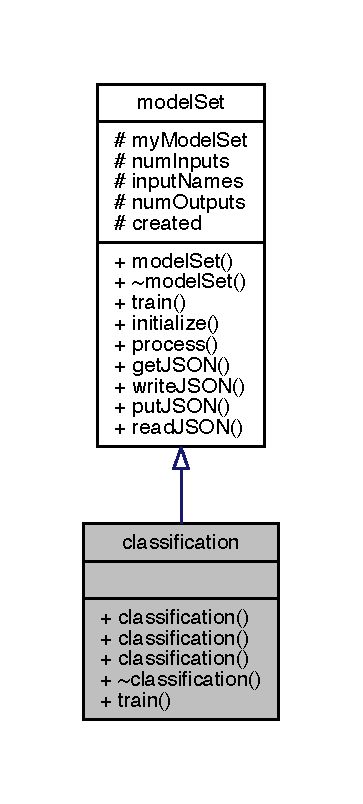
\includegraphics[width=168pt]{classclassification__inherit__graph}
\end{center}
\end{figure}


Collaboration diagram for classification\+:
\nopagebreak
\begin{figure}[H]
\begin{center}
\leavevmode
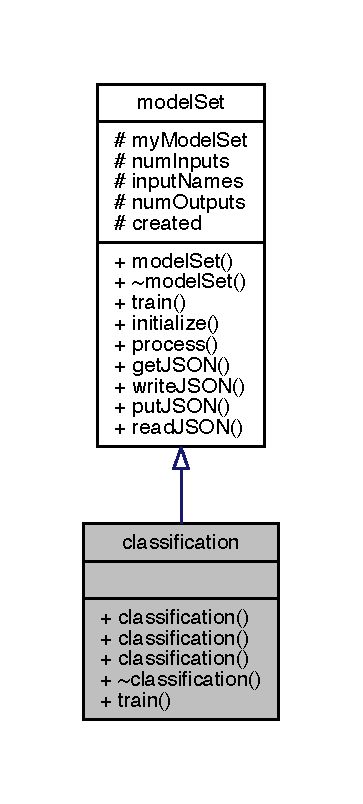
\includegraphics[width=168pt]{classclassification__coll__graph}
\end{center}
\end{figure}
\subsection*{Public Member Functions}
\begin{DoxyCompactItemize}
\item 
\hyperlink{classclassification_a96cfefed3bbc9b8b61a44b9c6cc9e29a}{classification} ()
\item 
\hyperlink{classclassification_a825ef0d6ba9ba826d22969be72a9011f}{classification} (std\+::vector$<$ \hyperlink{structtraining_example}{training\+Example} $>$ training\+Set)
\item 
\hyperlink{classclassification_ab76d1e8c617be54ede9ea47dd3c128bf}{classification} (int num\+Inputs, int num\+Outputs)
\item 
bool \hyperlink{classclassification_a8e834c25309bc471c5bb8e8730874c82}{train} (std\+::vector$<$ \hyperlink{structtraining_example}{training\+Example} $>$ training\+Set)
\end{DoxyCompactItemize}
\subsection*{Additional Inherited Members}


\subsection{Detailed Description}
Class for implementing a set of classification models.

This doesn\textquotesingle{}t do anything \hyperlink{classmodel_set}{model\+Set} can\textquotesingle{}t do. But, it\textquotesingle{}s simpler and more like wekinator. 

\subsection{Constructor \& Destructor Documentation}
\mbox{\Hypertarget{classclassification_a96cfefed3bbc9b8b61a44b9c6cc9e29a}\label{classclassification_a96cfefed3bbc9b8b61a44b9c6cc9e29a}} 
\index{classification@{classification}!classification@{classification}}
\index{classification@{classification}!classification@{classification}}
\subsubsection{\texorpdfstring{classification()}{classification()}\hspace{0.1cm}{\footnotesize\ttfamily [1/3]}}
{\footnotesize\ttfamily classification\+::classification (\begin{DoxyParamCaption}{ }\end{DoxyParamCaption})}

with no arguments, just make an empty vector \mbox{\Hypertarget{classclassification_a825ef0d6ba9ba826d22969be72a9011f}\label{classclassification_a825ef0d6ba9ba826d22969be72a9011f}} 
\index{classification@{classification}!classification@{classification}}
\index{classification@{classification}!classification@{classification}}
\subsubsection{\texorpdfstring{classification()}{classification()}\hspace{0.1cm}{\footnotesize\ttfamily [2/3]}}
{\footnotesize\ttfamily classification\+::classification (\begin{DoxyParamCaption}\item[{std\+::vector$<$ \hyperlink{structtraining_example}{training\+Example} $>$}]{training\+Set }\end{DoxyParamCaption})}

create based on training set inputs and outputs \mbox{\Hypertarget{classclassification_ab76d1e8c617be54ede9ea47dd3c128bf}\label{classclassification_ab76d1e8c617be54ede9ea47dd3c128bf}} 
\index{classification@{classification}!classification@{classification}}
\index{classification@{classification}!classification@{classification}}
\subsubsection{\texorpdfstring{classification()}{classification()}\hspace{0.1cm}{\footnotesize\ttfamily [3/3]}}
{\footnotesize\ttfamily classification\+::classification (\begin{DoxyParamCaption}\item[{int}]{num\+Inputs,  }\item[{int}]{num\+Outputs }\end{DoxyParamCaption})}

create with proper models, but not trained 

\subsection{Member Function Documentation}
\mbox{\Hypertarget{classclassification_a8e834c25309bc471c5bb8e8730874c82}\label{classclassification_a8e834c25309bc471c5bb8e8730874c82}} 
\index{classification@{classification}!train@{train}}
\index{train@{train}!classification@{classification}}
\subsubsection{\texorpdfstring{train()}{train()}}
{\footnotesize\ttfamily bool classification\+::train (\begin{DoxyParamCaption}\item[{std\+::vector$<$ \hyperlink{structtraining_example}{training\+Example} $>$}]{training\+Set }\end{DoxyParamCaption})\hspace{0.3cm}{\ttfamily [virtual]}}

Train on a specified set, causes creation if not created 

Reimplemented from \hyperlink{classmodel_set_ab0b16ec988c8077158de1c3d8986df03}{model\+Set}.



The documentation for this class was generated from the following files\+:\begin{DoxyCompactItemize}
\item 
classification.\+h\item 
classification.\+cpp\end{DoxyCompactItemize}

\hypertarget{classknn_classification}{}\section{knn\+Classification Class Reference}
\label{classknn_classification}\index{knn\+Classification@{knn\+Classification}}


{\ttfamily \#include $<$knn\+Classification.\+h$>$}



Inheritance diagram for knn\+Classification\+:\nopagebreak
\begin{figure}[H]
\begin{center}
\leavevmode
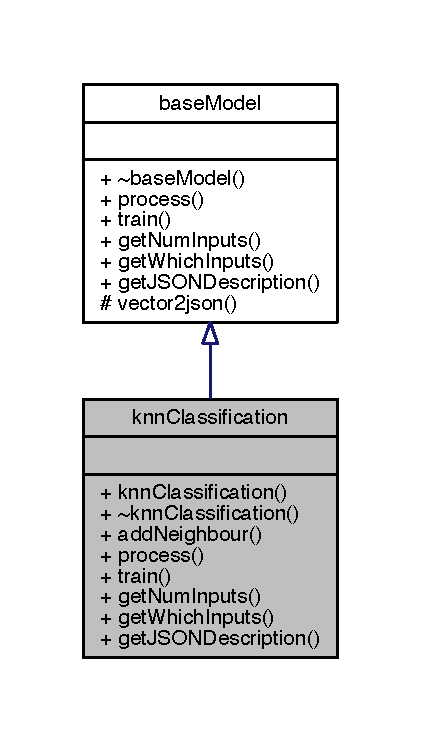
\includegraphics[width=202pt]{classknn_classification__inherit__graph}
\end{center}
\end{figure}


Collaboration diagram for knn\+Classification\+:\nopagebreak
\begin{figure}[H]
\begin{center}
\leavevmode
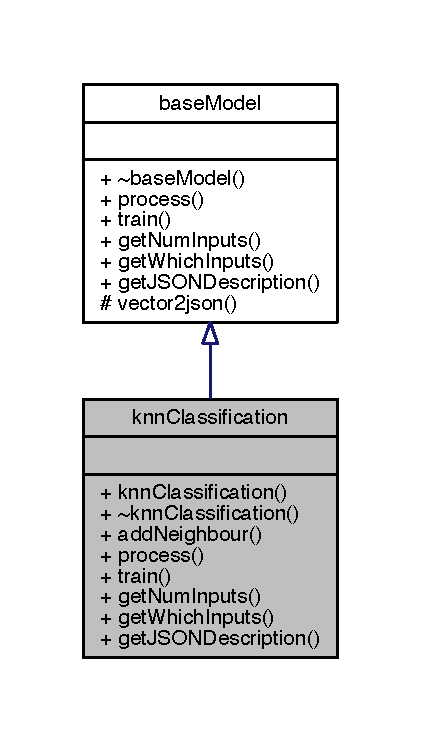
\includegraphics[width=202pt]{classknn_classification__coll__graph}
\end{center}
\end{figure}
\subsection*{Public Member Functions}
\begin{DoxyCompactItemize}
\item 
\hyperlink{classknn_classification_a93e0eda34ff02a37baaa8700b46ec5fd}{knn\+Classification} (int num\+\_\+inputs, std\+::vector$<$ int $>$ which\+\_\+inputs, std\+::vector$<$ \hyperlink{structtraining_example}{training\+Example} $>$ training\+Set, int k)
\item 
\hyperlink{classknn_classification_a37e034151bb6d69c3952454df630dd80}{$\sim$knn\+Classification} ()
\item 
void \hyperlink{classknn_classification_a591f953b182fed995ebfb13c712b76d5}{add\+Neighbour} (int, std\+::vector$<$ double $>$)
\item 
double \hyperlink{classknn_classification_a909050a125c4bf5cc2e48db0202fcb79}{process} (std\+::vector$<$ double $>$)
\item 
void \hyperlink{classknn_classification_ae159e53f542d08d04c76760f2e25e843}{train} (std\+::vector$<$ \hyperlink{structtraining_example}{training\+Example} $>$ training\+Set)
\item 
int \hyperlink{classknn_classification_a3f9c8fb78c6a66f0ab9440629140400d}{get\+Num\+Inputs} ()
\item 
std\+::vector$<$ int $>$ \hyperlink{classknn_classification_af7db9297f695e67df6af08719da37921}{get\+Which\+Inputs} ()
\item 
void \hyperlink{classknn_classification_a456b4b1b0fedb8f8fbe6d810bd80ceb8}{get\+J\+S\+O\+N\+Description} (Json\+::\+Value \&current\+Model)
\end{DoxyCompactItemize}
\subsection*{Additional Inherited Members}


\subsection{Detailed Description}
Class for implementing a knn classifier 

\subsection{Constructor \& Destructor Documentation}
\mbox{\Hypertarget{classknn_classification_a93e0eda34ff02a37baaa8700b46ec5fd}\label{classknn_classification_a93e0eda34ff02a37baaa8700b46ec5fd}} 
\index{knn\+Classification@{knn\+Classification}!knn\+Classification@{knn\+Classification}}
\index{knn\+Classification@{knn\+Classification}!knn\+Classification@{knn\+Classification}}
\subsubsection{\texorpdfstring{knn\+Classification()}{knnClassification()}}
{\footnotesize\ttfamily knn\+Classification\+::knn\+Classification (\begin{DoxyParamCaption}\item[{int}]{num\+\_\+inputs,  }\item[{std\+::vector$<$ int $>$}]{which\+\_\+inputs,  }\item[{std\+::vector$<$ \hyperlink{structtraining_example}{training\+Example} $>$}]{training\+Set,  }\item[{int}]{k }\end{DoxyParamCaption})}

Constructor that takes training examples in 
\begin{DoxyParams}{Parameters}
{\em number} & of inputs expected in the training and input vectors \\
\hline
{\em vector} & of input numbers to be fed into the classifer. \\
\hline
{\em vector} & of training examples \\
\hline
{\em how} & many near neighbours to evaluate \\
\hline
\end{DoxyParams}
\mbox{\Hypertarget{classknn_classification_a37e034151bb6d69c3952454df630dd80}\label{classknn_classification_a37e034151bb6d69c3952454df630dd80}} 
\index{knn\+Classification@{knn\+Classification}!````~knn\+Classification@{$\sim$knn\+Classification}}
\index{````~knn\+Classification@{$\sim$knn\+Classification}!knn\+Classification@{knn\+Classification}}
\subsubsection{\texorpdfstring{$\sim$knn\+Classification()}{~knnClassification()}}
{\footnotesize\ttfamily knn\+Classification\+::$\sim$knn\+Classification (\begin{DoxyParamCaption}{ }\end{DoxyParamCaption})}



\subsection{Member Function Documentation}
\mbox{\Hypertarget{classknn_classification_a591f953b182fed995ebfb13c712b76d5}\label{classknn_classification_a591f953b182fed995ebfb13c712b76d5}} 
\index{knn\+Classification@{knn\+Classification}!add\+Neighbour@{add\+Neighbour}}
\index{add\+Neighbour@{add\+Neighbour}!knn\+Classification@{knn\+Classification}}
\subsubsection{\texorpdfstring{add\+Neighbour()}{addNeighbour()}}
{\footnotesize\ttfamily void knn\+Classification\+::add\+Neighbour (\begin{DoxyParamCaption}\item[{int}]{class\+Num,  }\item[{std\+::vector$<$ double $>$}]{features }\end{DoxyParamCaption})}

add another example to the existing training set 
\begin{DoxyParams}{Parameters}
{\em class} & number of example \\
\hline
{\em feature} & vector of example \\
\hline
\end{DoxyParams}
\mbox{\Hypertarget{classknn_classification_a456b4b1b0fedb8f8fbe6d810bd80ceb8}\label{classknn_classification_a456b4b1b0fedb8f8fbe6d810bd80ceb8}} 
\index{knn\+Classification@{knn\+Classification}!get\+J\+S\+O\+N\+Description@{get\+J\+S\+O\+N\+Description}}
\index{get\+J\+S\+O\+N\+Description@{get\+J\+S\+O\+N\+Description}!knn\+Classification@{knn\+Classification}}
\subsubsection{\texorpdfstring{get\+J\+S\+O\+N\+Description()}{getJSONDescription()}}
{\footnotesize\ttfamily void knn\+Classification\+::get\+J\+S\+O\+N\+Description (\begin{DoxyParamCaption}\item[{Json\+::\+Value \&}]{current\+Model }\end{DoxyParamCaption})\hspace{0.3cm}{\ttfamily [virtual]}}



Implements \hyperlink{classbase_model_a54c7ba2132721c2f990ea2fe2313f863}{base\+Model}.

\mbox{\Hypertarget{classknn_classification_a3f9c8fb78c6a66f0ab9440629140400d}\label{classknn_classification_a3f9c8fb78c6a66f0ab9440629140400d}} 
\index{knn\+Classification@{knn\+Classification}!get\+Num\+Inputs@{get\+Num\+Inputs}}
\index{get\+Num\+Inputs@{get\+Num\+Inputs}!knn\+Classification@{knn\+Classification}}
\subsubsection{\texorpdfstring{get\+Num\+Inputs()}{getNumInputs()}}
{\footnotesize\ttfamily int knn\+Classification\+::get\+Num\+Inputs (\begin{DoxyParamCaption}{ }\end{DoxyParamCaption})\hspace{0.3cm}{\ttfamily [virtual]}}



Implements \hyperlink{classbase_model_a1601088280ebe5be525fd1fe49d4b1e1}{base\+Model}.

\mbox{\Hypertarget{classknn_classification_af7db9297f695e67df6af08719da37921}\label{classknn_classification_af7db9297f695e67df6af08719da37921}} 
\index{knn\+Classification@{knn\+Classification}!get\+Which\+Inputs@{get\+Which\+Inputs}}
\index{get\+Which\+Inputs@{get\+Which\+Inputs}!knn\+Classification@{knn\+Classification}}
\subsubsection{\texorpdfstring{get\+Which\+Inputs()}{getWhichInputs()}}
{\footnotesize\ttfamily std\+::vector$<$ int $>$ knn\+Classification\+::get\+Which\+Inputs (\begin{DoxyParamCaption}{ }\end{DoxyParamCaption})\hspace{0.3cm}{\ttfamily [virtual]}}



Implements \hyperlink{classbase_model_a5d6b7579536f5713eed0b7b4a6687a16}{base\+Model}.

\mbox{\Hypertarget{classknn_classification_a909050a125c4bf5cc2e48db0202fcb79}\label{classknn_classification_a909050a125c4bf5cc2e48db0202fcb79}} 
\index{knn\+Classification@{knn\+Classification}!process@{process}}
\index{process@{process}!knn\+Classification@{knn\+Classification}}
\subsubsection{\texorpdfstring{process()}{process()}}
{\footnotesize\ttfamily double knn\+Classification\+::process (\begin{DoxyParamCaption}\item[{std\+::vector$<$ double $>$}]{input\+Vector }\end{DoxyParamCaption})\hspace{0.3cm}{\ttfamily [virtual]}}

Generate an output value from a single input vector. 
\begin{DoxyParams}{Parameters}
{\em A} & standard vector of doubles to be evaluated. \\
\hline
\end{DoxyParams}
\begin{DoxyReturn}{Returns}
A single double\+: the nearest class as determined by k-\/nearest neighbor. 
\end{DoxyReturn}


Implements \hyperlink{classbase_model_a07d92b944728ff2b3339d6bceaecb6a3}{base\+Model}.

\mbox{\Hypertarget{classknn_classification_ae159e53f542d08d04c76760f2e25e843}\label{classknn_classification_ae159e53f542d08d04c76760f2e25e843}} 
\index{knn\+Classification@{knn\+Classification}!train@{train}}
\index{train@{train}!knn\+Classification@{knn\+Classification}}
\subsubsection{\texorpdfstring{train()}{train()}}
{\footnotesize\ttfamily void knn\+Classification\+::train (\begin{DoxyParamCaption}\item[{std\+::vector$<$ \hyperlink{structtraining_example}{training\+Example} $>$}]{training\+Set }\end{DoxyParamCaption})\hspace{0.3cm}{\ttfamily [virtual]}}

Fill the model with a vector of examples.


\begin{DoxyParams}{Parameters}
{\em The} & training set is a vector of training examples that contain both a vector of input values and a double specifying desired output class. \\
\hline
\end{DoxyParams}


Implements \hyperlink{classbase_model_aed9192d6c0f17a1816a55b077baf2523}{base\+Model}.



The documentation for this class was generated from the following files\+:\begin{DoxyCompactItemize}
\item 
\hyperlink{knn_classification_8h}{knn\+Classification.\+h}\item 
\hyperlink{knn_classification_8cpp}{knn\+Classification.\+cpp}\end{DoxyCompactItemize}

\hypertarget{classmodel_set}{}\section{model\+Set Class Reference}
\label{classmodel_set}\index{model\+Set@{model\+Set}}


{\ttfamily \#include $<$model\+Set.\+h$>$}



Inheritance diagram for model\+Set\+:\nopagebreak
\begin{figure}[H]
\begin{center}
\leavevmode
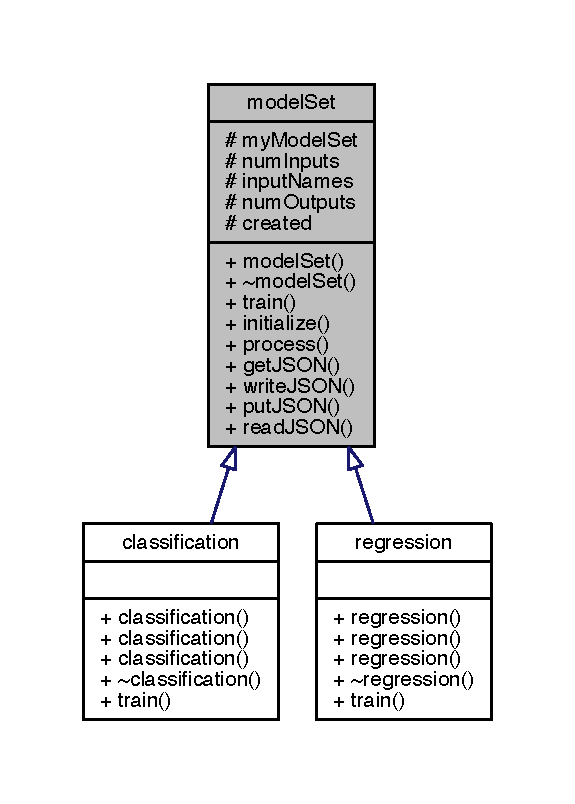
\includegraphics[width=264pt]{classmodel_set__inherit__graph}
\end{center}
\end{figure}


Collaboration diagram for model\+Set\+:\nopagebreak
\begin{figure}[H]
\begin{center}
\leavevmode
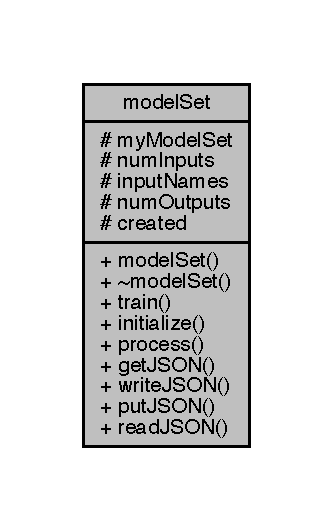
\includegraphics[width=160pt]{classmodel_set__coll__graph}
\end{center}
\end{figure}
\subsection*{Public Member Functions}
\begin{DoxyCompactItemize}
\item 
\hyperlink{classmodel_set_ae44cba85f4c52e7d05e0f622b3ea9030}{model\+Set} ()
\item 
\hyperlink{classmodel_set_a21eadb6e6cdd54dda57a4a94582bfe7b}{$\sim$model\+Set} ()
\item 
virtual bool \hyperlink{classmodel_set_ab0b16ec988c8077158de1c3d8986df03}{train} (std\+::vector$<$ \hyperlink{structtraining_example}{training\+Example} $>$ training\+Set)
\item 
bool \hyperlink{classmodel_set_afefb50a0fe8f45821c6a7599784d7eb4}{initialize} ()
\item 
std\+::vector$<$ double $>$ \hyperlink{classmodel_set_a232b11aa2987dd7db56c0f55edf868ea}{process} (std\+::vector$<$ double $>$ input\+Vector)
\item 
std\+::string \hyperlink{classmodel_set_a031987885b1462ec7d7dbeef0c803d97}{get\+J\+S\+ON} ()
\item 
void \hyperlink{classmodel_set_a805879b6c8ec54d16c2ac511c72442b9}{write\+J\+S\+ON} (std\+::string filepath)
\item 
bool \hyperlink{classmodel_set_a09b07168fbe9d9377eb26f30bf16884c}{put\+J\+S\+ON} (std\+::string json\+Message)
\item 
bool \hyperlink{classmodel_set_a8f7a837515889c6bddb3184a022b1727}{read\+J\+S\+ON} (std\+::string filepath)
\end{DoxyCompactItemize}
\subsection*{Protected Attributes}
\begin{DoxyCompactItemize}
\item 
std\+::vector$<$ \hyperlink{classbase_model}{base\+Model} $\ast$ $>$ \hyperlink{classmodel_set_a390b0b864a8e727f481537b3c37aa721}{my\+Model\+Set}
\item 
int \hyperlink{classmodel_set_ad10fbc1228a85f1200cb89589ad92755}{num\+Inputs}
\item 
std\+::vector$<$ std\+::string $>$ \hyperlink{classmodel_set_ab4b67d7dbdf0659ba6bd18af7247e2ad}{input\+Names}
\item 
int \hyperlink{classmodel_set_addc0df56b9f1970c9816050634933716}{num\+Outputs}
\item 
bool \hyperlink{classmodel_set_a0029dc6f8ccfd77353ad38b48198ad7d}{created}
\end{DoxyCompactItemize}


\subsection{Detailed Description}
This class holds a set of models with the same or different algorithms. 

\subsection{Constructor \& Destructor Documentation}
\mbox{\Hypertarget{classmodel_set_ae44cba85f4c52e7d05e0f622b3ea9030}\label{classmodel_set_ae44cba85f4c52e7d05e0f622b3ea9030}} 
\index{model\+Set@{model\+Set}!model\+Set@{model\+Set}}
\index{model\+Set@{model\+Set}!model\+Set@{model\+Set}}
\subsubsection{\texorpdfstring{model\+Set()}{modelSet()}}
{\footnotesize\ttfamily model\+Set\+::model\+Set (\begin{DoxyParamCaption}{ }\end{DoxyParamCaption})}

No arguments, don\textquotesingle{}t create any models yet \mbox{\Hypertarget{classmodel_set_a21eadb6e6cdd54dda57a4a94582bfe7b}\label{classmodel_set_a21eadb6e6cdd54dda57a4a94582bfe7b}} 
\index{model\+Set@{model\+Set}!````~model\+Set@{$\sim$model\+Set}}
\index{````~model\+Set@{$\sim$model\+Set}!model\+Set@{model\+Set}}
\subsubsection{\texorpdfstring{$\sim$model\+Set()}{~modelSet()}}
{\footnotesize\ttfamily model\+Set\+::$\sim$model\+Set (\begin{DoxyParamCaption}{ }\end{DoxyParamCaption})}



\subsection{Member Function Documentation}
\mbox{\Hypertarget{classmodel_set_a031987885b1462ec7d7dbeef0c803d97}\label{classmodel_set_a031987885b1462ec7d7dbeef0c803d97}} 
\index{model\+Set@{model\+Set}!get\+J\+S\+ON@{get\+J\+S\+ON}}
\index{get\+J\+S\+ON@{get\+J\+S\+ON}!model\+Set@{model\+Set}}
\subsubsection{\texorpdfstring{get\+J\+S\+O\+N()}{getJSON()}}
{\footnotesize\ttfamily std\+::string model\+Set\+::get\+J\+S\+ON (\begin{DoxyParamCaption}{ }\end{DoxyParamCaption})}

Get a J\+S\+ON representation of the model in the form of a styled string \mbox{\Hypertarget{classmodel_set_afefb50a0fe8f45821c6a7599784d7eb4}\label{classmodel_set_afefb50a0fe8f45821c6a7599784d7eb4}} 
\index{model\+Set@{model\+Set}!initialize@{initialize}}
\index{initialize@{initialize}!model\+Set@{model\+Set}}
\subsubsection{\texorpdfstring{initialize()}{initialize()}}
{\footnotesize\ttfamily bool model\+Set\+::initialize (\begin{DoxyParamCaption}{ }\end{DoxyParamCaption})}

reset to pre-\/training state \mbox{\Hypertarget{classmodel_set_a232b11aa2987dd7db56c0f55edf868ea}\label{classmodel_set_a232b11aa2987dd7db56c0f55edf868ea}} 
\index{model\+Set@{model\+Set}!process@{process}}
\index{process@{process}!model\+Set@{model\+Set}}
\subsubsection{\texorpdfstring{process()}{process()}}
{\footnotesize\ttfamily std\+::vector$<$ double $>$ model\+Set\+::process (\begin{DoxyParamCaption}\item[{std\+::vector$<$ double $>$}]{input\+Vector }\end{DoxyParamCaption})}

run regression or classification for each model \mbox{\Hypertarget{classmodel_set_a09b07168fbe9d9377eb26f30bf16884c}\label{classmodel_set_a09b07168fbe9d9377eb26f30bf16884c}} 
\index{model\+Set@{model\+Set}!put\+J\+S\+ON@{put\+J\+S\+ON}}
\index{put\+J\+S\+ON@{put\+J\+S\+ON}!model\+Set@{model\+Set}}
\subsubsection{\texorpdfstring{put\+J\+S\+O\+N()}{putJSON()}}
{\footnotesize\ttfamily bool model\+Set\+::put\+J\+S\+ON (\begin{DoxyParamCaption}\item[{std\+::string}]{json\+Message }\end{DoxyParamCaption})}

configure empty model with string. See \hyperlink{classmodel_set_a031987885b1462ec7d7dbeef0c803d97}{get\+J\+S\+O\+N()} \mbox{\Hypertarget{classmodel_set_a8f7a837515889c6bddb3184a022b1727}\label{classmodel_set_a8f7a837515889c6bddb3184a022b1727}} 
\index{model\+Set@{model\+Set}!read\+J\+S\+ON@{read\+J\+S\+ON}}
\index{read\+J\+S\+ON@{read\+J\+S\+ON}!model\+Set@{model\+Set}}
\subsubsection{\texorpdfstring{read\+J\+S\+O\+N()}{readJSON()}}
{\footnotesize\ttfamily bool model\+Set\+::read\+J\+S\+ON (\begin{DoxyParamCaption}\item[{std\+::string}]{filepath }\end{DoxyParamCaption})}

read a J\+S\+ON file at file path and build a \hyperlink{classmodel_set}{model\+Set} from it \mbox{\Hypertarget{classmodel_set_ab0b16ec988c8077158de1c3d8986df03}\label{classmodel_set_ab0b16ec988c8077158de1c3d8986df03}} 
\index{model\+Set@{model\+Set}!train@{train}}
\index{train@{train}!model\+Set@{model\+Set}}
\subsubsection{\texorpdfstring{train()}{train()}}
{\footnotesize\ttfamily bool model\+Set\+::train (\begin{DoxyParamCaption}\item[{std\+::vector$<$ \hyperlink{structtraining_example}{training\+Example} $>$}]{training\+Set }\end{DoxyParamCaption})\hspace{0.3cm}{\ttfamily [virtual]}}

Train on a specified set, causes creation if not created 

Reimplemented in \hyperlink{classclassification_a8e834c25309bc471c5bb8e8730874c82}{classification}, and \hyperlink{classregression_ae45d7dbf24cab75202d966d116829813}{regression}.

\mbox{\Hypertarget{classmodel_set_a805879b6c8ec54d16c2ac511c72442b9}\label{classmodel_set_a805879b6c8ec54d16c2ac511c72442b9}} 
\index{model\+Set@{model\+Set}!write\+J\+S\+ON@{write\+J\+S\+ON}}
\index{write\+J\+S\+ON@{write\+J\+S\+ON}!model\+Set@{model\+Set}}
\subsubsection{\texorpdfstring{write\+J\+S\+O\+N()}{writeJSON()}}
{\footnotesize\ttfamily void model\+Set\+::write\+J\+S\+ON (\begin{DoxyParamCaption}\item[{std\+::string}]{filepath }\end{DoxyParamCaption})}

Write a J\+S\+ON model description to specified file path 

\subsection{Member Data Documentation}
\mbox{\Hypertarget{classmodel_set_a0029dc6f8ccfd77353ad38b48198ad7d}\label{classmodel_set_a0029dc6f8ccfd77353ad38b48198ad7d}} 
\index{model\+Set@{model\+Set}!created@{created}}
\index{created@{created}!model\+Set@{model\+Set}}
\subsubsection{\texorpdfstring{created}{created}}
{\footnotesize\ttfamily bool model\+Set\+::created\hspace{0.3cm}{\ttfamily [protected]}}

\mbox{\Hypertarget{classmodel_set_ab4b67d7dbdf0659ba6bd18af7247e2ad}\label{classmodel_set_ab4b67d7dbdf0659ba6bd18af7247e2ad}} 
\index{model\+Set@{model\+Set}!input\+Names@{input\+Names}}
\index{input\+Names@{input\+Names}!model\+Set@{model\+Set}}
\subsubsection{\texorpdfstring{input\+Names}{inputNames}}
{\footnotesize\ttfamily std\+::vector$<$std\+::string$>$ model\+Set\+::input\+Names\hspace{0.3cm}{\ttfamily [protected]}}

\mbox{\Hypertarget{classmodel_set_a390b0b864a8e727f481537b3c37aa721}\label{classmodel_set_a390b0b864a8e727f481537b3c37aa721}} 
\index{model\+Set@{model\+Set}!my\+Model\+Set@{my\+Model\+Set}}
\index{my\+Model\+Set@{my\+Model\+Set}!model\+Set@{model\+Set}}
\subsubsection{\texorpdfstring{my\+Model\+Set}{myModelSet}}
{\footnotesize\ttfamily std\+::vector$<$\hyperlink{classbase_model}{base\+Model}$\ast$$>$ model\+Set\+::my\+Model\+Set\hspace{0.3cm}{\ttfamily [protected]}}

\mbox{\Hypertarget{classmodel_set_ad10fbc1228a85f1200cb89589ad92755}\label{classmodel_set_ad10fbc1228a85f1200cb89589ad92755}} 
\index{model\+Set@{model\+Set}!num\+Inputs@{num\+Inputs}}
\index{num\+Inputs@{num\+Inputs}!model\+Set@{model\+Set}}
\subsubsection{\texorpdfstring{num\+Inputs}{numInputs}}
{\footnotesize\ttfamily int model\+Set\+::num\+Inputs\hspace{0.3cm}{\ttfamily [protected]}}

\mbox{\Hypertarget{classmodel_set_addc0df56b9f1970c9816050634933716}\label{classmodel_set_addc0df56b9f1970c9816050634933716}} 
\index{model\+Set@{model\+Set}!num\+Outputs@{num\+Outputs}}
\index{num\+Outputs@{num\+Outputs}!model\+Set@{model\+Set}}
\subsubsection{\texorpdfstring{num\+Outputs}{numOutputs}}
{\footnotesize\ttfamily int model\+Set\+::num\+Outputs\hspace{0.3cm}{\ttfamily [protected]}}



The documentation for this class was generated from the following files\+:\begin{DoxyCompactItemize}
\item 
\hyperlink{model_set_8h}{model\+Set.\+h}\item 
\hyperlink{model_set_8cpp}{model\+Set.\+cpp}\end{DoxyCompactItemize}

\hypertarget{classneural_network}{}\section{neural\+Network Class Reference}
\label{classneural_network}\index{neural\+Network@{neural\+Network}}


{\ttfamily \#include $<$neural\+Network.\+h$>$}



Inheritance diagram for neural\+Network\+:
\nopagebreak
\begin{figure}[H]
\begin{center}
\leavevmode
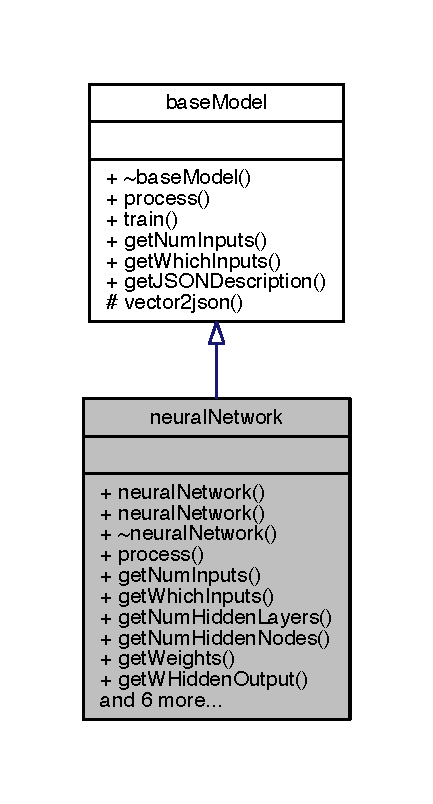
\includegraphics[width=208pt]{classneural_network__inherit__graph}
\end{center}
\end{figure}


Collaboration diagram for neural\+Network\+:
\nopagebreak
\begin{figure}[H]
\begin{center}
\leavevmode
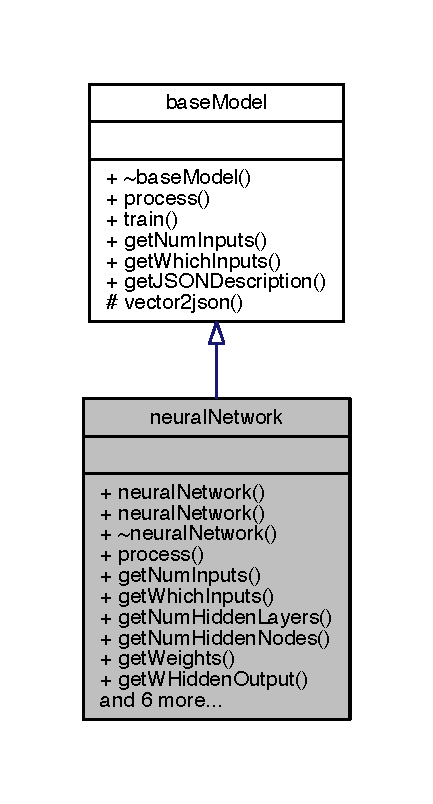
\includegraphics[width=208pt]{classneural_network__coll__graph}
\end{center}
\end{figure}
\subsection*{Public Member Functions}
\begin{DoxyCompactItemize}
\item 
\hyperlink{classneural_network_aee6fd482cd0b6b4004759bb57d4b14db}{neural\+Network} (int num\+\_\+inputs, std\+::vector$<$ int $>$ which\+\_\+inputs, int num\+\_\+hidden\+\_\+layers, int num\+\_\+hidden\+\_\+nodes, std\+::vector$<$ double $>$, std\+::vector$<$ double $>$, std\+::vector$<$ double $>$, std\+::vector$<$ double $>$, double, double)
\item 
\hyperlink{classneural_network_ad5cad1e6ac86745ab47fceeb8d42cbd9}{neural\+Network} (int num\+\_\+inputs, std\+::vector$<$ int $>$ which\+\_\+inputs, int num\+\_\+hidden\+\_\+layer, int num\+\_\+hidden\+\_\+nodes)
\item 
\hyperlink{classneural_network_a0967982cb0345a610f78d225d812086f}{$\sim$neural\+Network} ()
\item 
double \hyperlink{classneural_network_a2da76293dbe590594e79e96768c02a29}{process} (std\+::vector$<$ double $>$ input\+Vector)
\item 
\mbox{\Hypertarget{classneural_network_aaf9ff8b1a88126fcffc1e9f07a4ffe49}\label{classneural_network_aaf9ff8b1a88126fcffc1e9f07a4ffe49}} 
int {\bfseries get\+Num\+Inputs} ()
\item 
\mbox{\Hypertarget{classneural_network_afc93cb28c3897d4d1faa4ac8fbf0c1f8}\label{classneural_network_afc93cb28c3897d4d1faa4ac8fbf0c1f8}} 
std\+::vector$<$ int $>$ {\bfseries get\+Which\+Inputs} ()
\item 
\mbox{\Hypertarget{classneural_network_ade72f91a9207f52618f9b70cb585a992}\label{classneural_network_ade72f91a9207f52618f9b70cb585a992}} 
int {\bfseries get\+Num\+Hidden\+Layers} ()
\item 
\mbox{\Hypertarget{classneural_network_a679a628a34f70dd52f781c8c9dbd1a02}\label{classneural_network_a679a628a34f70dd52f781c8c9dbd1a02}} 
int {\bfseries get\+Num\+Hidden\+Nodes} ()
\item 
\mbox{\Hypertarget{classneural_network_a9822cd69469d7b2a946a9f87c8bebe5f}\label{classneural_network_a9822cd69469d7b2a946a9f87c8bebe5f}} 
std\+::vector$<$ double $>$ {\bfseries get\+Weights} ()
\item 
\mbox{\Hypertarget{classneural_network_ac372190f6eabf0af27e5c317f2a1d51b}\label{classneural_network_ac372190f6eabf0af27e5c317f2a1d51b}} 
std\+::vector$<$ double $>$ {\bfseries get\+W\+Hidden\+Output} ()
\item 
\mbox{\Hypertarget{classneural_network_a876638749a0c7027e82da294947f1840}\label{classneural_network_a876638749a0c7027e82da294947f1840}} 
std\+::vector$<$ double $>$ {\bfseries get\+In\+Ranges} ()
\item 
\mbox{\Hypertarget{classneural_network_af3fdc1c2bdf4794680ccc4cd845fb47e}\label{classneural_network_af3fdc1c2bdf4794680ccc4cd845fb47e}} 
std\+::vector$<$ double $>$ {\bfseries get\+In\+Bases} ()
\item 
\mbox{\Hypertarget{classneural_network_a9890f2967b4442eda4087869c57bccfd}\label{classneural_network_a9890f2967b4442eda4087869c57bccfd}} 
double {\bfseries get\+Out\+Range} ()
\item 
\mbox{\Hypertarget{classneural_network_a4524958a9de02bd5e48d0c991d634788}\label{classneural_network_a4524958a9de02bd5e48d0c991d634788}} 
double {\bfseries get\+Out\+Base} ()
\item 
\mbox{\Hypertarget{classneural_network_a83f5c57ed3f555cd534a6f4ea425dfb7}\label{classneural_network_a83f5c57ed3f555cd534a6f4ea425dfb7}} 
void {\bfseries get\+J\+S\+O\+N\+Description} (Json\+::\+Value \&current\+Model)
\item 
void \hyperlink{classneural_network_aae35def98392b0d0a51f2c82afc48efc}{train} (std\+::vector$<$ \hyperlink{structtraining_example}{training\+Example} $>$ training\+Set)
\end{DoxyCompactItemize}
\subsection*{Additional Inherited Members}


\subsection{Detailed Description}
Class for implementing a Neural Network.

This class includes both running and training, and constructors for reading trained models from J\+S\+ON. 

\subsection{Constructor \& Destructor Documentation}
\mbox{\Hypertarget{classneural_network_aee6fd482cd0b6b4004759bb57d4b14db}\label{classneural_network_aee6fd482cd0b6b4004759bb57d4b14db}} 
\index{neural\+Network@{neural\+Network}!neural\+Network@{neural\+Network}}
\index{neural\+Network@{neural\+Network}!neural\+Network@{neural\+Network}}
\subsubsection{\texorpdfstring{neural\+Network()}{neuralNetwork()}\hspace{0.1cm}{\footnotesize\ttfamily [1/2]}}
{\footnotesize\ttfamily neural\+Network\+::neural\+Network (\begin{DoxyParamCaption}\item[{int}]{num\+\_\+inputs,  }\item[{std\+::vector$<$ int $>$}]{which\+\_\+inputs,  }\item[{int}]{num\+\_\+hidden\+\_\+layers,  }\item[{int}]{num\+\_\+hidden\+\_\+nodes,  }\item[{std\+::vector$<$ double $>$}]{\+\_\+weights,  }\item[{std\+::vector$<$ double $>$}]{w\+\_\+hidden\+\_\+output,  }\item[{std\+::vector$<$ double $>$}]{in\+\_\+ranges,  }\item[{std\+::vector$<$ double $>$}]{in\+\_\+bases,  }\item[{double}]{out\+\_\+range,  }\item[{double}]{out\+\_\+base }\end{DoxyParamCaption})}

This is the constructor for building a trained model from J\+S\+ON. \mbox{\Hypertarget{classneural_network_ad5cad1e6ac86745ab47fceeb8d42cbd9}\label{classneural_network_ad5cad1e6ac86745ab47fceeb8d42cbd9}} 
\index{neural\+Network@{neural\+Network}!neural\+Network@{neural\+Network}}
\index{neural\+Network@{neural\+Network}!neural\+Network@{neural\+Network}}
\subsubsection{\texorpdfstring{neural\+Network()}{neuralNetwork()}\hspace{0.1cm}{\footnotesize\ttfamily [2/2]}}
{\footnotesize\ttfamily neural\+Network\+::neural\+Network (\begin{DoxyParamCaption}\item[{int}]{num\+\_\+inputs,  }\item[{std\+::vector$<$ int $>$}]{which\+\_\+inputs,  }\item[{int}]{num\+\_\+hidden\+\_\+layers,  }\item[{int}]{num\+\_\+hidden\+\_\+nodes }\end{DoxyParamCaption})}

This constructor creates a neural network that needs to be trained.


\begin{DoxyParams}{Parameters}
{\em num\+\_\+inputs} & is the number of inputs the network will process \\
\hline
{\em which\+\_\+inputs} & is an vector of which values in the input vector are being fed to the network. ex\+: \{0,2,4\} \\
\hline
{\em num\+\_\+hidden\+\_\+layer} & is the number of hidden layers in the network. Must be at least 1. \\
\hline
{\em num\+\_\+hidden\+\_\+nodes} & is the number of hidden nodes in each hidden layer. Often, this is the same as num\+\_\+inputs\\
\hline
\end{DoxyParams}
\begin{DoxyReturn}{Returns}
A \hyperlink{classneural_network}{neural\+Network} instance with randomized weights and no normalization values. These will be set or adjusted during training.
\end{DoxyReturn}
This is the constructor for a model that needs to be trained. \mbox{\Hypertarget{classneural_network_a0967982cb0345a610f78d225d812086f}\label{classneural_network_a0967982cb0345a610f78d225d812086f}} 
\index{neural\+Network@{neural\+Network}!````~neural\+Network@{$\sim$neural\+Network}}
\index{````~neural\+Network@{$\sim$neural\+Network}!neural\+Network@{neural\+Network}}
\subsubsection{\texorpdfstring{$\sim$neural\+Network()}{~neuralNetwork()}}
{\footnotesize\ttfamily neural\+Network\+::$\sim$neural\+Network (\begin{DoxyParamCaption}{ }\end{DoxyParamCaption})}

This destructor is not needed. 

\subsection{Member Function Documentation}
\mbox{\Hypertarget{classneural_network_a2da76293dbe590594e79e96768c02a29}\label{classneural_network_a2da76293dbe590594e79e96768c02a29}} 
\index{neural\+Network@{neural\+Network}!process@{process}}
\index{process@{process}!neural\+Network@{neural\+Network}}
\subsubsection{\texorpdfstring{process()}{process()}}
{\footnotesize\ttfamily double neural\+Network\+::process (\begin{DoxyParamCaption}\item[{std\+::vector$<$ double $>$}]{input\+Vector }\end{DoxyParamCaption})\hspace{0.3cm}{\ttfamily [virtual]}}

Generate an output value from a single input vector. 
\begin{DoxyParams}{Parameters}
{\em A} & standard vector of doubles that feed-\/forward regression will run on. \\
\hline
\end{DoxyParams}
\begin{DoxyReturn}{Returns}
A single double, which is the result of the feed-\/forward operation 
\end{DoxyReturn}


Implements \hyperlink{classbase_model}{base\+Model}.

\mbox{\Hypertarget{classneural_network_aae35def98392b0d0a51f2c82afc48efc}\label{classneural_network_aae35def98392b0d0a51f2c82afc48efc}} 
\index{neural\+Network@{neural\+Network}!train@{train}}
\index{train@{train}!neural\+Network@{neural\+Network}}
\subsubsection{\texorpdfstring{train()}{train()}}
{\footnotesize\ttfamily void neural\+Network\+::train (\begin{DoxyParamCaption}\item[{std\+::vector$<$ \hyperlink{structtraining_example}{training\+Example} $>$}]{training\+Set }\end{DoxyParamCaption})\hspace{0.3cm}{\ttfamily [virtual]}}

These pertain to the training, and aren\textquotesingle{}t need to run a trained model Train a model using backpropagation.


\begin{DoxyParams}{Parameters}
{\em The} & training set is a vector of training examples that contain both a vector of input values and a double specifying desired output. \\
\hline
\end{DoxyParams}


Implements \hyperlink{classbase_model}{base\+Model}.



The documentation for this class was generated from the following files\+:\begin{DoxyCompactItemize}
\item 
neural\+Network.\+h\item 
neural\+Network.\+cpp\end{DoxyCompactItemize}

\hypertarget{classregression}{}\section{regression Class Reference}
\label{classregression}\index{regression@{regression}}


{\ttfamily \#include $<$regression.\+h$>$}



Inheritance diagram for regression\+:\nopagebreak
\begin{figure}[H]
\begin{center}
\leavevmode
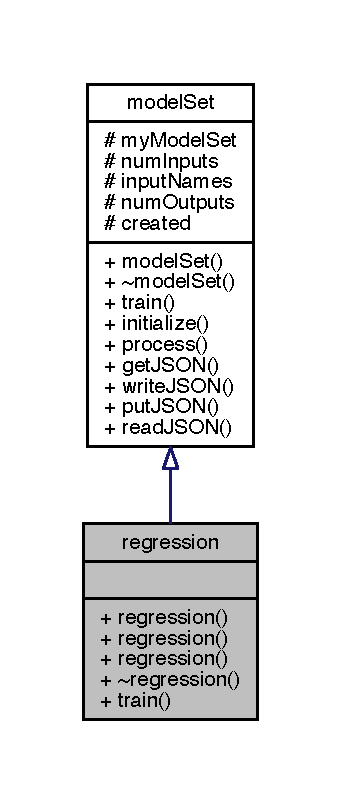
\includegraphics[width=160pt]{classregression__inherit__graph}
\end{center}
\end{figure}


Collaboration diagram for regression\+:\nopagebreak
\begin{figure}[H]
\begin{center}
\leavevmode
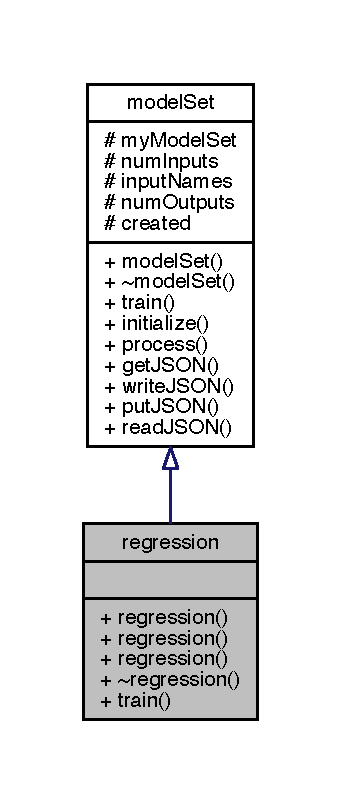
\includegraphics[width=160pt]{classregression__coll__graph}
\end{center}
\end{figure}
\subsection*{Public Member Functions}
\begin{DoxyCompactItemize}
\item 
\hyperlink{classregression_a40993153659b1f637cf4d596df6e97ab}{regression} ()
\item 
\hyperlink{classregression_ad03f74e09d96f315de3933628e8f4138}{regression} (std\+::vector$<$ \hyperlink{structtraining_example}{training\+Example} $>$ training\+Set)
\item 
\hyperlink{classregression_a9d38dcda0e5c99caf0faf85f98a5ebb3}{regression} (int \hyperlink{classmodel_set_ad10fbc1228a85f1200cb89589ad92755}{num\+Inputs}, int \hyperlink{classmodel_set_addc0df56b9f1970c9816050634933716}{num\+Outputs})
\item 
bool \hyperlink{classregression_ae45d7dbf24cab75202d966d116829813}{train} (std\+::vector$<$ \hyperlink{structtraining_example}{training\+Example} $>$ training\+Set)
\end{DoxyCompactItemize}
\subsection*{Additional Inherited Members}


\subsection{Detailed Description}
Class for implementing a set of regression models.

This doesn\textquotesingle{}t do anything \hyperlink{classmodel_set}{model\+Set} can\textquotesingle{}t do. But, it\textquotesingle{}s simpler and more like wekinator. 

\subsection{Constructor \& Destructor Documentation}
\mbox{\Hypertarget{classregression_a40993153659b1f637cf4d596df6e97ab}\label{classregression_a40993153659b1f637cf4d596df6e97ab}} 
\index{regression@{regression}!regression@{regression}}
\index{regression@{regression}!regression@{regression}}
\subsubsection{\texorpdfstring{regression()}{regression()}\hspace{0.1cm}{\footnotesize\ttfamily [1/3]}}
{\footnotesize\ttfamily regression\+::regression (\begin{DoxyParamCaption}{ }\end{DoxyParamCaption})}

with no arguments, just make an empty vector \mbox{\Hypertarget{classregression_ad03f74e09d96f315de3933628e8f4138}\label{classregression_ad03f74e09d96f315de3933628e8f4138}} 
\index{regression@{regression}!regression@{regression}}
\index{regression@{regression}!regression@{regression}}
\subsubsection{\texorpdfstring{regression()}{regression()}\hspace{0.1cm}{\footnotesize\ttfamily [2/3]}}
{\footnotesize\ttfamily regression\+::regression (\begin{DoxyParamCaption}\item[{std\+::vector$<$ \hyperlink{structtraining_example}{training\+Example} $>$}]{training\+Set }\end{DoxyParamCaption})}

create based on training set inputs and outputs \mbox{\Hypertarget{classregression_a9d38dcda0e5c99caf0faf85f98a5ebb3}\label{classregression_a9d38dcda0e5c99caf0faf85f98a5ebb3}} 
\index{regression@{regression}!regression@{regression}}
\index{regression@{regression}!regression@{regression}}
\subsubsection{\texorpdfstring{regression()}{regression()}\hspace{0.1cm}{\footnotesize\ttfamily [3/3]}}
{\footnotesize\ttfamily regression\+::regression (\begin{DoxyParamCaption}\item[{int}]{num\+Inputs,  }\item[{int}]{num\+Outputs }\end{DoxyParamCaption})}

create with proper models, but not trained 

\subsection{Member Function Documentation}
\mbox{\Hypertarget{classregression_ae45d7dbf24cab75202d966d116829813}\label{classregression_ae45d7dbf24cab75202d966d116829813}} 
\index{regression@{regression}!train@{train}}
\index{train@{train}!regression@{regression}}
\subsubsection{\texorpdfstring{train()}{train()}}
{\footnotesize\ttfamily bool regression\+::train (\begin{DoxyParamCaption}\item[{std\+::vector$<$ \hyperlink{structtraining_example}{training\+Example} $>$}]{training\+Set }\end{DoxyParamCaption})\hspace{0.3cm}{\ttfamily [virtual]}}

Train on a specified set, causes creation if not created 

Reimplemented from \hyperlink{classmodel_set_ab0b16ec988c8077158de1c3d8986df03}{model\+Set}.



The documentation for this class was generated from the following files\+:\begin{DoxyCompactItemize}
\item 
\hyperlink{regression_8h}{regression.\+h}\item 
\hyperlink{regression_8cpp}{regression.\+cpp}\end{DoxyCompactItemize}

\hypertarget{structtraining_example}{}\section{training\+Example Struct Reference}
\label{structtraining_example}\index{training\+Example@{training\+Example}}


{\ttfamily \#include $<$training\+Example.\+h$>$}



Collaboration diagram for training\+Example\+:\nopagebreak
\begin{figure}[H]
\begin{center}
\leavevmode
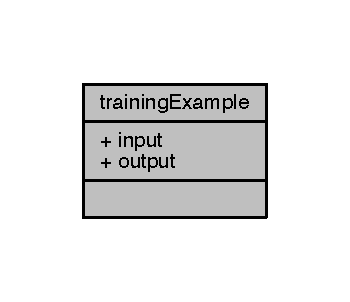
\includegraphics[width=168pt]{structtraining_example__coll__graph}
\end{center}
\end{figure}
\subsection*{Public Attributes}
\begin{DoxyCompactItemize}
\item 
std\+::vector$<$ double $>$ \hyperlink{structtraining_example_a066378f49152305e496c0f76fb13246d}{input}
\item 
std\+::vector$<$ double $>$ \hyperlink{structtraining_example_ae776963ea692ba5260d4d329f579c9fd}{output}
\end{DoxyCompactItemize}


\subsection{Detailed Description}
This is used by both NN and K\+NN models for training 

\subsection{Member Data Documentation}
\mbox{\Hypertarget{structtraining_example_a066378f49152305e496c0f76fb13246d}\label{structtraining_example_a066378f49152305e496c0f76fb13246d}} 
\index{training\+Example@{training\+Example}!input@{input}}
\index{input@{input}!training\+Example@{training\+Example}}
\subsubsection{\texorpdfstring{input}{input}}
{\footnotesize\ttfamily std\+::vector$<$double$>$ training\+Example\+::input}

\mbox{\Hypertarget{structtraining_example_ae776963ea692ba5260d4d329f579c9fd}\label{structtraining_example_ae776963ea692ba5260d4d329f579c9fd}} 
\index{training\+Example@{training\+Example}!output@{output}}
\index{output@{output}!training\+Example@{training\+Example}}
\subsubsection{\texorpdfstring{output}{output}}
{\footnotesize\ttfamily std\+::vector$<$double$>$ training\+Example\+::output}



The documentation for this struct was generated from the following file\+:\begin{DoxyCompactItemize}
\item 
\hyperlink{training_example_8h}{training\+Example.\+h}\end{DoxyCompactItemize}

\chapter{File Documentation}
\hypertarget{base_model_8h}{}\section{base\+Model.\+h File Reference}
\label{base_model_8h}\index{base\+Model.\+h@{base\+Model.\+h}}
{\ttfamily \#include $<$vector$>$}\newline
{\ttfamily \#include \char`\"{}training\+Example.\+h\char`\"{}}\newline
{\ttfamily \#include \char`\"{}json.\+h\char`\"{}}\newline
Include dependency graph for base\+Model.\+h\+:\nopagebreak
\begin{figure}[H]
\begin{center}
\leavevmode
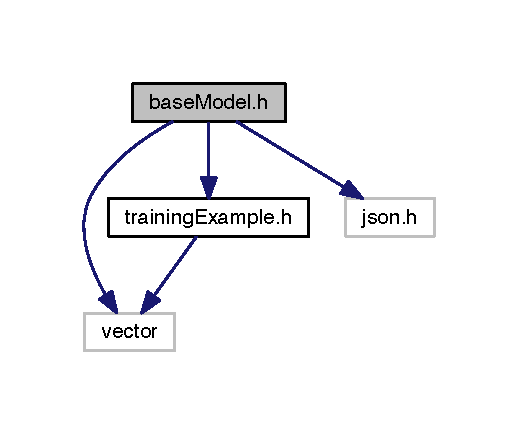
\includegraphics[width=249pt]{base_model_8h__incl}
\end{center}
\end{figure}
This graph shows which files directly or indirectly include this file\+:\nopagebreak
\begin{figure}[H]
\begin{center}
\leavevmode
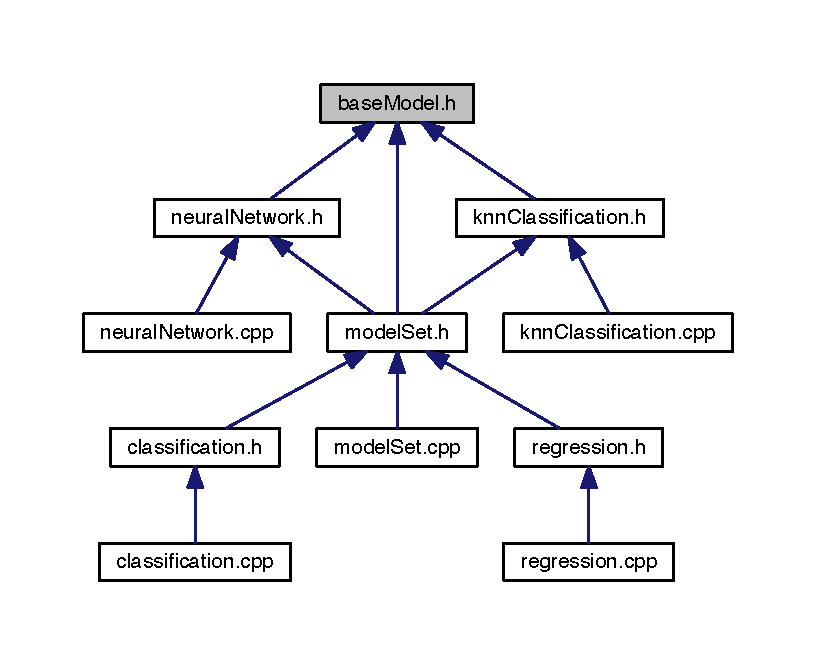
\includegraphics[width=350pt]{base_model_8h__dep__incl}
\end{center}
\end{figure}
\subsection*{Classes}
\begin{DoxyCompactItemize}
\item 
class \hyperlink{classbase_model}{base\+Model}
\end{DoxyCompactItemize}

\hypertarget{classification_8cpp}{}\section{classification.\+cpp File Reference}
\label{classification_8cpp}\index{classification.\+cpp@{classification.\+cpp}}
{\ttfamily \#include $<$vector$>$}\newline
{\ttfamily \#include \char`\"{}classification.\+h\char`\"{}}\newline
Include dependency graph for classification.\+cpp\+:\nopagebreak
\begin{figure}[H]
\begin{center}
\leavevmode
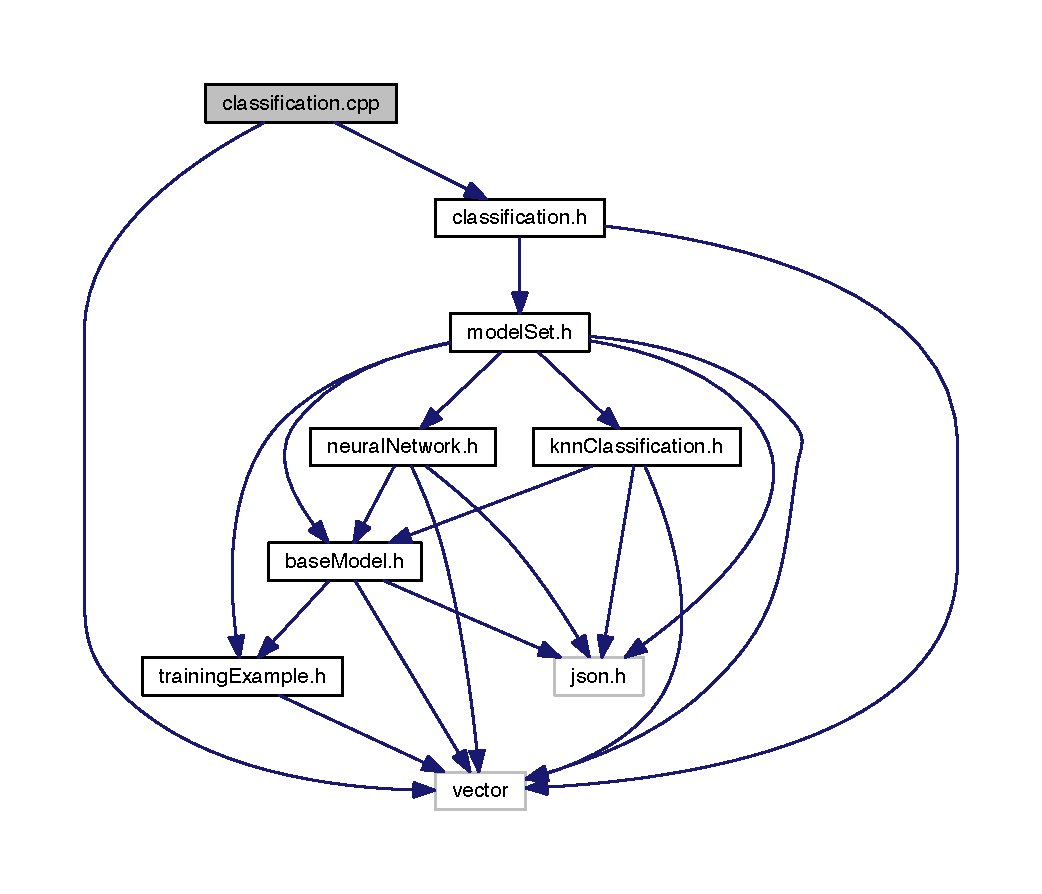
\includegraphics[width=350pt]{classification_8cpp__incl}
\end{center}
\end{figure}

\hypertarget{classification_8h}{}\section{classification.\+h File Reference}
\label{classification_8h}\index{classification.\+h@{classification.\+h}}
{\ttfamily \#include $<$vector$>$}\newline
{\ttfamily \#include \char`\"{}model\+Set.\+h\char`\"{}}\newline
Include dependency graph for classification.\+h\+:\nopagebreak
\begin{figure}[H]
\begin{center}
\leavevmode
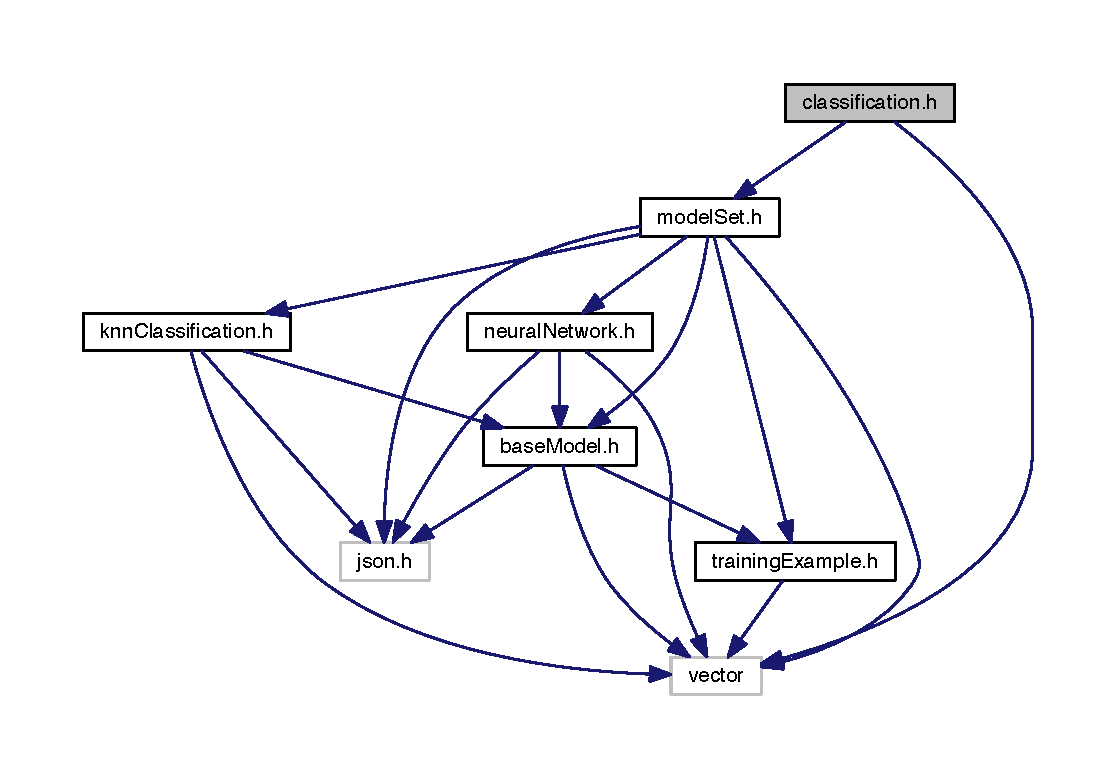
\includegraphics[width=350pt]{classification_8h__incl}
\end{center}
\end{figure}
This graph shows which files directly or indirectly include this file\+:\nopagebreak
\begin{figure}[H]
\begin{center}
\leavevmode
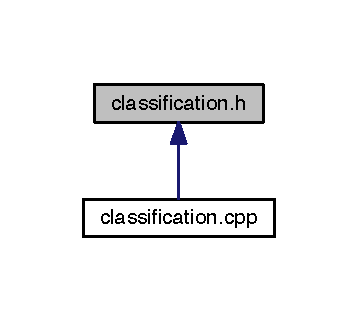
\includegraphics[width=172pt]{classification_8h__dep__incl}
\end{center}
\end{figure}
\subsection*{Classes}
\begin{DoxyCompactItemize}
\item 
class \hyperlink{classclassification}{classification}
\end{DoxyCompactItemize}

\hypertarget{classification_embindings_8h}{}\section{classification\+Embindings.\+h File Reference}
\label{classification_embindings_8h}\index{classification\+Embindings.\+h@{classification\+Embindings.\+h}}
{\ttfamily \#include $<$emscripten.\+h$>$}\newline
{\ttfamily \#include $<$bind.\+h$>$}\newline
Include dependency graph for classification\+Embindings.\+h\+:\nopagebreak
\begin{figure}[H]
\begin{center}
\leavevmode
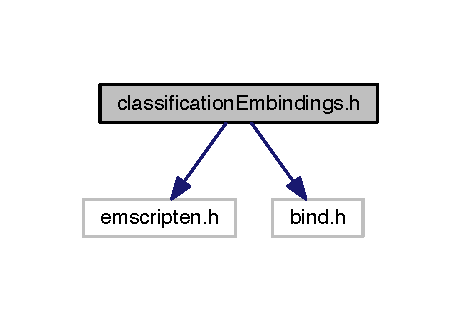
\includegraphics[width=221pt]{classification_embindings_8h__incl}
\end{center}
\end{figure}
\subsection*{Functions}
\begin{DoxyCompactItemize}
\item 
\hyperlink{classification_embindings_8h_a58dacb6aae53224a343bc2a20f44a4c5}{E\+M\+S\+C\+R\+I\+P\+T\+E\+N\+\_\+\+B\+I\+N\+D\+I\+N\+GS} (classification\+\_\+module)
\end{DoxyCompactItemize}


\subsection{Function Documentation}
\mbox{\Hypertarget{classification_embindings_8h_a58dacb6aae53224a343bc2a20f44a4c5}\label{classification_embindings_8h_a58dacb6aae53224a343bc2a20f44a4c5}} 
\index{classification\+Embindings.\+h@{classification\+Embindings.\+h}!E\+M\+S\+C\+R\+I\+P\+T\+E\+N\+\_\+\+B\+I\+N\+D\+I\+N\+GS@{E\+M\+S\+C\+R\+I\+P\+T\+E\+N\+\_\+\+B\+I\+N\+D\+I\+N\+GS}}
\index{E\+M\+S\+C\+R\+I\+P\+T\+E\+N\+\_\+\+B\+I\+N\+D\+I\+N\+GS@{E\+M\+S\+C\+R\+I\+P\+T\+E\+N\+\_\+\+B\+I\+N\+D\+I\+N\+GS}!classification\+Embindings.\+h@{classification\+Embindings.\+h}}
\subsubsection{\texorpdfstring{E\+M\+S\+C\+R\+I\+P\+T\+E\+N\+\_\+\+B\+I\+N\+D\+I\+N\+G\+S()}{EMSCRIPTEN\_BINDINGS()}}
{\footnotesize\ttfamily E\+M\+S\+C\+R\+I\+P\+T\+E\+N\+\_\+\+B\+I\+N\+D\+I\+N\+GS (\begin{DoxyParamCaption}\item[{classification\+\_\+module}]{ }\end{DoxyParamCaption})}


\hypertarget{knn_classification_8cpp}{}\section{knn\+Classification.\+cpp File Reference}
\label{knn_classification_8cpp}\index{knn\+Classification.\+cpp@{knn\+Classification.\+cpp}}
{\ttfamily \#include $<$cmath$>$}\newline
{\ttfamily \#include $<$utility$>$}\newline
{\ttfamily \#include $<$map$>$}\newline
{\ttfamily \#include $<$vector$>$}\newline
{\ttfamily \#include \char`\"{}knn\+Classification.\+h\char`\"{}}\newline
Include dependency graph for knn\+Classification.\+cpp\+:\nopagebreak
\begin{figure}[H]
\begin{center}
\leavevmode
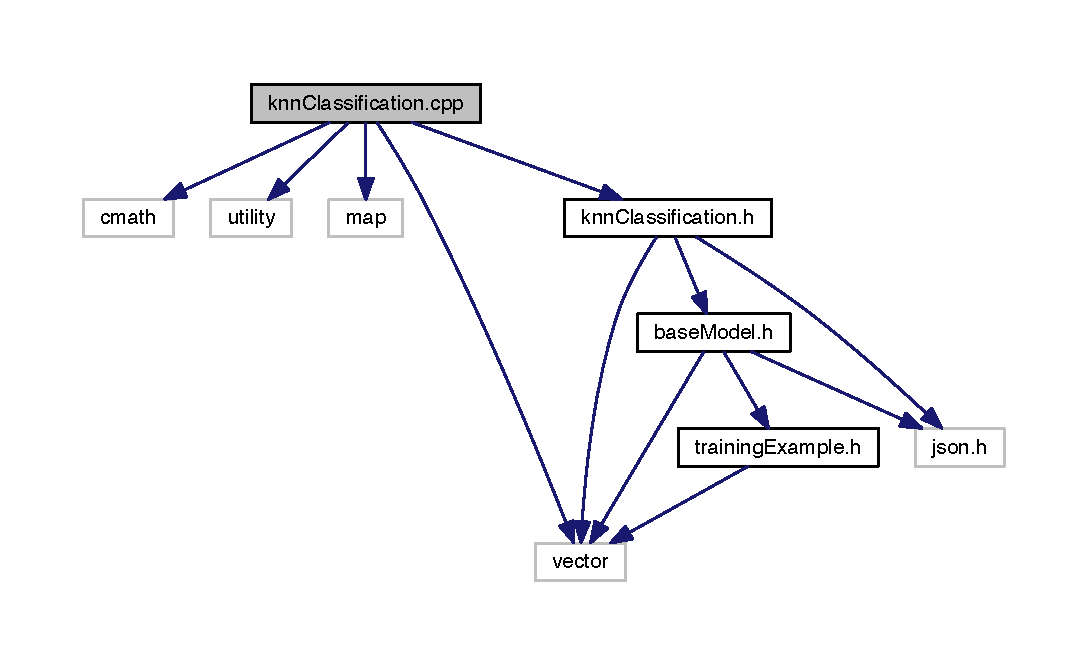
\includegraphics[width=350pt]{knn_classification_8cpp__incl}
\end{center}
\end{figure}

\hypertarget{knn_classification_8h}{}\section{knn\+Classification.\+h File Reference}
\label{knn_classification_8h}\index{knn\+Classification.\+h@{knn\+Classification.\+h}}
{\ttfamily \#include $<$vector$>$}\newline
{\ttfamily \#include \char`\"{}base\+Model.\+h\char`\"{}}\newline
{\ttfamily \#include \char`\"{}json.\+h\char`\"{}}\newline
Include dependency graph for knn\+Classification.\+h\+:\nopagebreak
\begin{figure}[H]
\begin{center}
\leavevmode
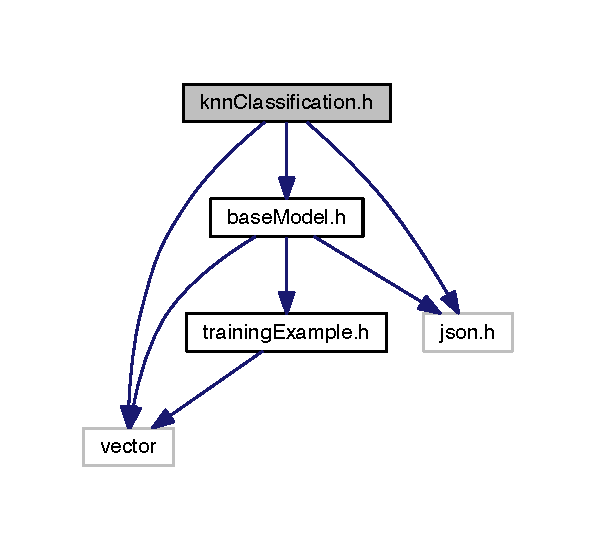
\includegraphics[width=286pt]{knn_classification_8h__incl}
\end{center}
\end{figure}
This graph shows which files directly or indirectly include this file\+:\nopagebreak
\begin{figure}[H]
\begin{center}
\leavevmode
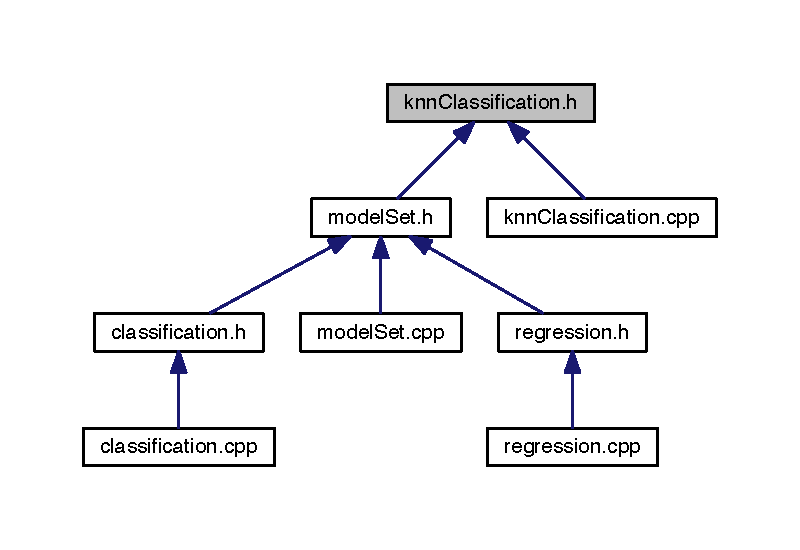
\includegraphics[width=350pt]{knn_classification_8h__dep__incl}
\end{center}
\end{figure}
\subsection*{Classes}
\begin{DoxyCompactItemize}
\item 
class \hyperlink{classknn_classification}{knn\+Classification}
\end{DoxyCompactItemize}

\hypertarget{knn_embindings_8h}{}\section{knn\+Embindings.\+h File Reference}
\label{knn_embindings_8h}\index{knn\+Embindings.\+h@{knn\+Embindings.\+h}}
{\ttfamily \#include $<$vector$>$}\newline
{\ttfamily \#include $<$emscripten.\+h$>$}\newline
{\ttfamily \#include $<$bind.\+h$>$}\newline
Include dependency graph for knn\+Embindings.\+h\+:\nopagebreak
\begin{figure}[H]
\begin{center}
\leavevmode
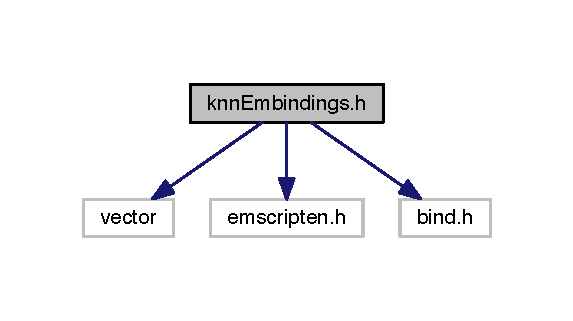
\includegraphics[width=275pt]{knn_embindings_8h__incl}
\end{center}
\end{figure}
\subsection*{Functions}
\begin{DoxyCompactItemize}
\item 
\hyperlink{knn_embindings_8h_acea9cc23407d20afe27e8fa64adc4c20}{E\+M\+S\+C\+R\+I\+P\+T\+E\+N\+\_\+\+B\+I\+N\+D\+I\+N\+GS} (stl\+\_\+wrappers)
\item 
\hyperlink{knn_embindings_8h_addf8b6205f8e8cb85d07921c65354a4d}{E\+M\+S\+C\+R\+I\+P\+T\+E\+N\+\_\+\+B\+I\+N\+D\+I\+N\+GS} (knn\+\_\+module)
\end{DoxyCompactItemize}


\subsection{Function Documentation}
\mbox{\Hypertarget{knn_embindings_8h_acea9cc23407d20afe27e8fa64adc4c20}\label{knn_embindings_8h_acea9cc23407d20afe27e8fa64adc4c20}} 
\index{knn\+Embindings.\+h@{knn\+Embindings.\+h}!E\+M\+S\+C\+R\+I\+P\+T\+E\+N\+\_\+\+B\+I\+N\+D\+I\+N\+GS@{E\+M\+S\+C\+R\+I\+P\+T\+E\+N\+\_\+\+B\+I\+N\+D\+I\+N\+GS}}
\index{E\+M\+S\+C\+R\+I\+P\+T\+E\+N\+\_\+\+B\+I\+N\+D\+I\+N\+GS@{E\+M\+S\+C\+R\+I\+P\+T\+E\+N\+\_\+\+B\+I\+N\+D\+I\+N\+GS}!knn\+Embindings.\+h@{knn\+Embindings.\+h}}
\subsubsection{\texorpdfstring{E\+M\+S\+C\+R\+I\+P\+T\+E\+N\+\_\+\+B\+I\+N\+D\+I\+N\+G\+S()}{EMSCRIPTEN\_BINDINGS()}\hspace{0.1cm}{\footnotesize\ttfamily [1/2]}}
{\footnotesize\ttfamily E\+M\+S\+C\+R\+I\+P\+T\+E\+N\+\_\+\+B\+I\+N\+D\+I\+N\+GS (\begin{DoxyParamCaption}\item[{stl\+\_\+wrappers}]{ }\end{DoxyParamCaption})}

\mbox{\Hypertarget{knn_embindings_8h_addf8b6205f8e8cb85d07921c65354a4d}\label{knn_embindings_8h_addf8b6205f8e8cb85d07921c65354a4d}} 
\index{knn\+Embindings.\+h@{knn\+Embindings.\+h}!E\+M\+S\+C\+R\+I\+P\+T\+E\+N\+\_\+\+B\+I\+N\+D\+I\+N\+GS@{E\+M\+S\+C\+R\+I\+P\+T\+E\+N\+\_\+\+B\+I\+N\+D\+I\+N\+GS}}
\index{E\+M\+S\+C\+R\+I\+P\+T\+E\+N\+\_\+\+B\+I\+N\+D\+I\+N\+GS@{E\+M\+S\+C\+R\+I\+P\+T\+E\+N\+\_\+\+B\+I\+N\+D\+I\+N\+GS}!knn\+Embindings.\+h@{knn\+Embindings.\+h}}
\subsubsection{\texorpdfstring{E\+M\+S\+C\+R\+I\+P\+T\+E\+N\+\_\+\+B\+I\+N\+D\+I\+N\+G\+S()}{EMSCRIPTEN\_BINDINGS()}\hspace{0.1cm}{\footnotesize\ttfamily [2/2]}}
{\footnotesize\ttfamily E\+M\+S\+C\+R\+I\+P\+T\+E\+N\+\_\+\+B\+I\+N\+D\+I\+N\+GS (\begin{DoxyParamCaption}\item[{knn\+\_\+module}]{ }\end{DoxyParamCaption})}


\hypertarget{model_set_8cpp}{}\section{model\+Set.\+cpp File Reference}
\label{model_set_8cpp}\index{model\+Set.\+cpp@{model\+Set.\+cpp}}
{\ttfamily \#include $<$iostream$>$}\newline
{\ttfamily \#include $<$fstream$>$}\newline
{\ttfamily \#include $<$vector$>$}\newline
{\ttfamily \#include $<$cmath$>$}\newline
{\ttfamily \#include \char`\"{}model\+Set.\+h\char`\"{}}\newline
{\ttfamily \#include \char`\"{}json.\+h\char`\"{}}\newline
Include dependency graph for model\+Set.\+cpp\+:\nopagebreak
\begin{figure}[H]
\begin{center}
\leavevmode
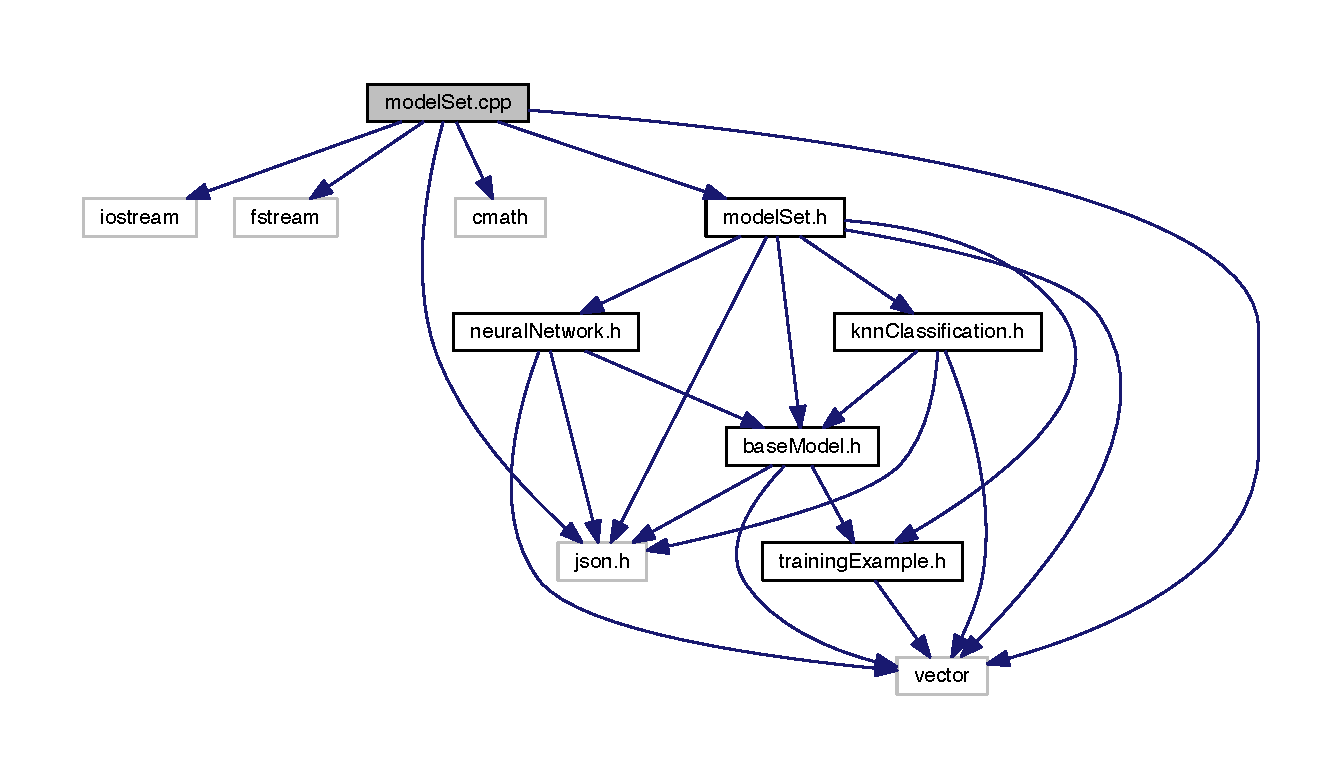
\includegraphics[width=350pt]{model_set_8cpp__incl}
\end{center}
\end{figure}
\subsection*{Functions}
\begin{DoxyCompactItemize}
\item 
std\+::vector$<$ double $>$ \hyperlink{model_set_8cpp_a16b102f78151b1c7aab2671b4b69f988}{json2vector} (Json\+::\+Value json)
\end{DoxyCompactItemize}


\subsection{Function Documentation}
\mbox{\Hypertarget{model_set_8cpp_a16b102f78151b1c7aab2671b4b69f988}\label{model_set_8cpp_a16b102f78151b1c7aab2671b4b69f988}} 
\index{model\+Set.\+cpp@{model\+Set.\+cpp}!json2vector@{json2vector}}
\index{json2vector@{json2vector}!model\+Set.\+cpp@{model\+Set.\+cpp}}
\subsubsection{\texorpdfstring{json2vector()}{json2vector()}}
{\footnotesize\ttfamily std\+::vector$<$double$>$ json2vector (\begin{DoxyParamCaption}\item[{Json\+::\+Value}]{json }\end{DoxyParamCaption})}


\hypertarget{model_set_8h}{}\section{model\+Set.\+h File Reference}
\label{model_set_8h}\index{model\+Set.\+h@{model\+Set.\+h}}
{\ttfamily \#include $<$vector$>$}\newline
{\ttfamily \#include \char`\"{}training\+Example.\+h\char`\"{}}\newline
{\ttfamily \#include \char`\"{}base\+Model.\+h\char`\"{}}\newline
{\ttfamily \#include \char`\"{}neural\+Network.\+h\char`\"{}}\newline
{\ttfamily \#include \char`\"{}knn\+Classification.\+h\char`\"{}}\newline
{\ttfamily \#include \char`\"{}json.\+h\char`\"{}}\newline
Include dependency graph for model\+Set.\+h\+:\nopagebreak
\begin{figure}[H]
\begin{center}
\leavevmode
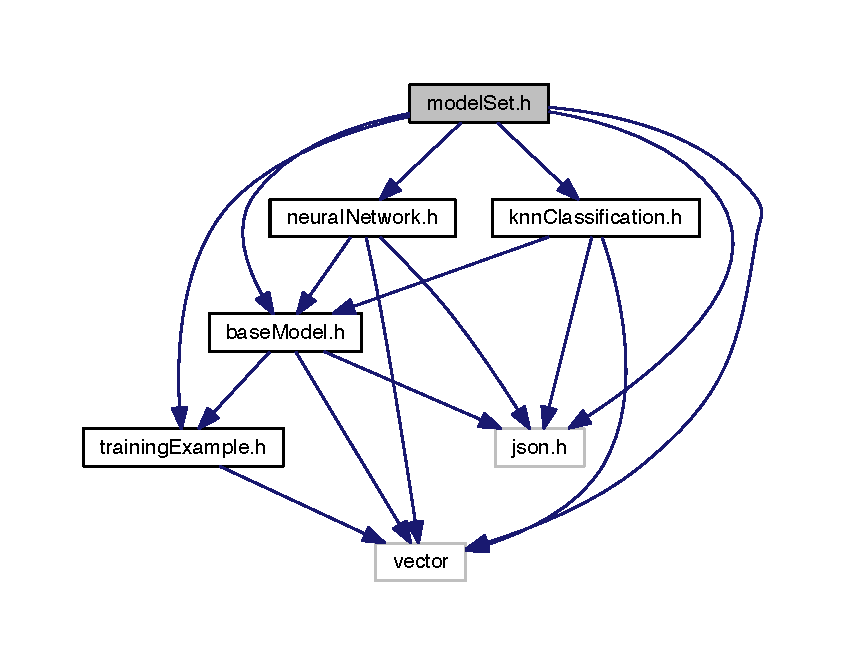
\includegraphics[width=350pt]{model_set_8h__incl}
\end{center}
\end{figure}
This graph shows which files directly or indirectly include this file\+:\nopagebreak
\begin{figure}[H]
\begin{center}
\leavevmode
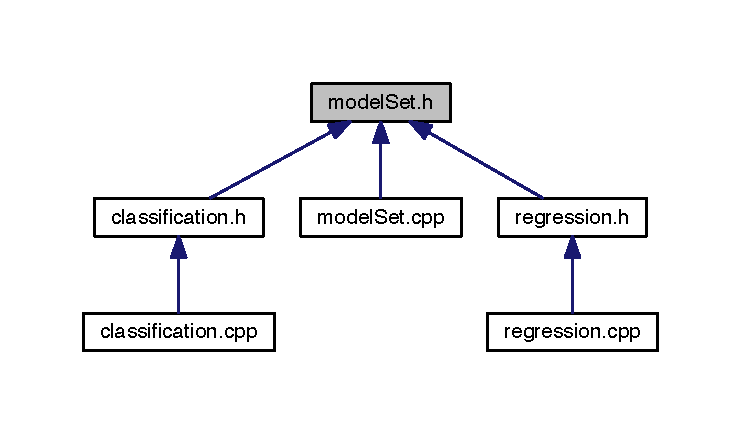
\includegraphics[width=350pt]{model_set_8h__dep__incl}
\end{center}
\end{figure}
\subsection*{Classes}
\begin{DoxyCompactItemize}
\item 
class \hyperlink{classmodel_set}{model\+Set}
\end{DoxyCompactItemize}

\hypertarget{model_set_embindings_8h}{}\section{model\+Set\+Embindings.\+h File Reference}
\label{model_set_embindings_8h}\index{model\+Set\+Embindings.\+h@{model\+Set\+Embindings.\+h}}
{\ttfamily \#include $<$emscripten.\+h$>$}\newline
{\ttfamily \#include $<$bind.\+h$>$}\newline
Include dependency graph for model\+Set\+Embindings.\+h\+:\nopagebreak
\begin{figure}[H]
\begin{center}
\leavevmode
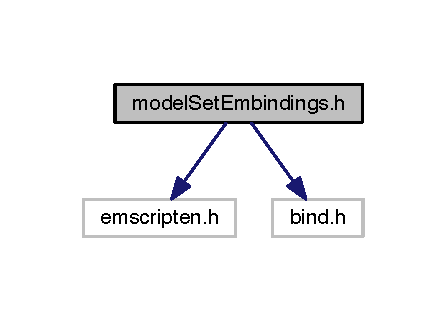
\includegraphics[width=214pt]{model_set_embindings_8h__incl}
\end{center}
\end{figure}
\subsection*{Functions}
\begin{DoxyCompactItemize}
\item 
\hyperlink{model_set_embindings_8h_a7c1c05b7d56f04ba6bf083bbac8f484e}{E\+M\+S\+C\+R\+I\+P\+T\+E\+N\+\_\+\+B\+I\+N\+D\+I\+N\+GS} (model\+Set\+\_\+module)
\end{DoxyCompactItemize}


\subsection{Function Documentation}
\mbox{\Hypertarget{model_set_embindings_8h_a7c1c05b7d56f04ba6bf083bbac8f484e}\label{model_set_embindings_8h_a7c1c05b7d56f04ba6bf083bbac8f484e}} 
\index{model\+Set\+Embindings.\+h@{model\+Set\+Embindings.\+h}!E\+M\+S\+C\+R\+I\+P\+T\+E\+N\+\_\+\+B\+I\+N\+D\+I\+N\+GS@{E\+M\+S\+C\+R\+I\+P\+T\+E\+N\+\_\+\+B\+I\+N\+D\+I\+N\+GS}}
\index{E\+M\+S\+C\+R\+I\+P\+T\+E\+N\+\_\+\+B\+I\+N\+D\+I\+N\+GS@{E\+M\+S\+C\+R\+I\+P\+T\+E\+N\+\_\+\+B\+I\+N\+D\+I\+N\+GS}!model\+Set\+Embindings.\+h@{model\+Set\+Embindings.\+h}}
\subsubsection{\texorpdfstring{E\+M\+S\+C\+R\+I\+P\+T\+E\+N\+\_\+\+B\+I\+N\+D\+I\+N\+G\+S()}{EMSCRIPTEN\_BINDINGS()}}
{\footnotesize\ttfamily E\+M\+S\+C\+R\+I\+P\+T\+E\+N\+\_\+\+B\+I\+N\+D\+I\+N\+GS (\begin{DoxyParamCaption}\item[{model\+Set\+\_\+module}]{ }\end{DoxyParamCaption})}


\hypertarget{neural_network_8cpp}{}\section{neural\+Network.\+cpp File Reference}
\label{neural_network_8cpp}\index{neural\+Network.\+cpp@{neural\+Network.\+cpp}}
{\ttfamily \#include $<$math.\+h$>$}\newline
{\ttfamily \#include $<$random$>$}\newline
{\ttfamily \#include $<$algorithm$>$}\newline
{\ttfamily \#include $<$vector$>$}\newline
{\ttfamily \#include \char`\"{}neural\+Network.\+h\char`\"{}}\newline
Include dependency graph for neural\+Network.\+cpp\+:\nopagebreak
\begin{figure}[H]
\begin{center}
\leavevmode
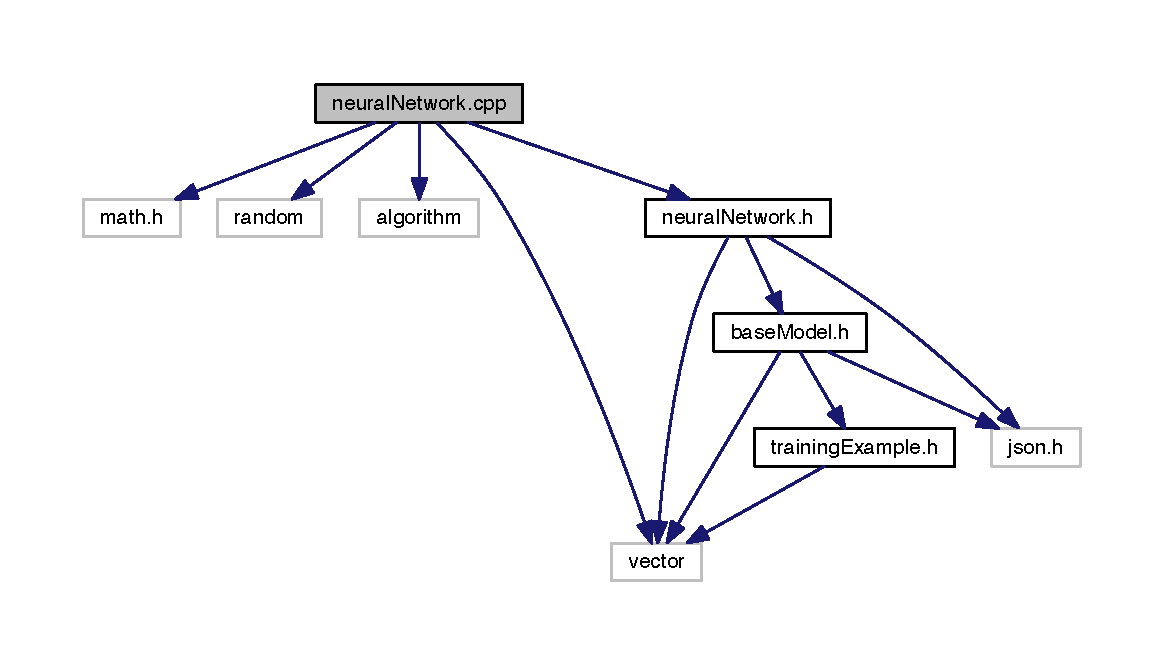
\includegraphics[width=350pt]{neural_network_8cpp__incl}
\end{center}
\end{figure}

\hypertarget{neural_network_8h}{}\section{neural\+Network.\+h File Reference}
\label{neural_network_8h}\index{neural\+Network.\+h@{neural\+Network.\+h}}
{\ttfamily \#include $<$vector$>$}\newline
{\ttfamily \#include \char`\"{}base\+Model.\+h\char`\"{}}\newline
{\ttfamily \#include \char`\"{}json.\+h\char`\"{}}\newline
Include dependency graph for neural\+Network.\+h\+:\nopagebreak
\begin{figure}[H]
\begin{center}
\leavevmode
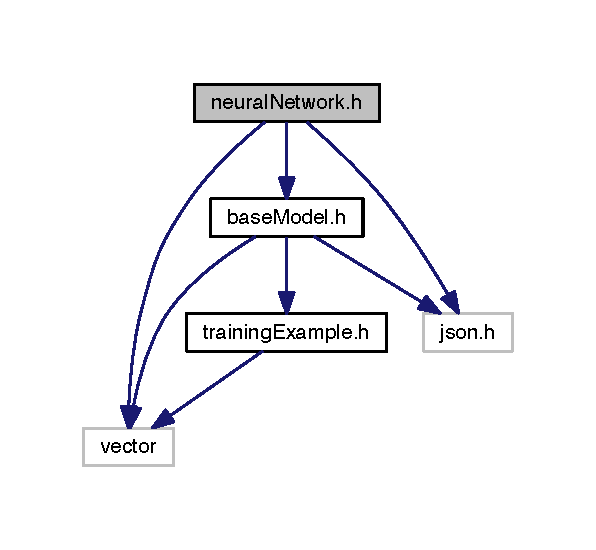
\includegraphics[width=286pt]{neural_network_8h__incl}
\end{center}
\end{figure}
This graph shows which files directly or indirectly include this file\+:\nopagebreak
\begin{figure}[H]
\begin{center}
\leavevmode
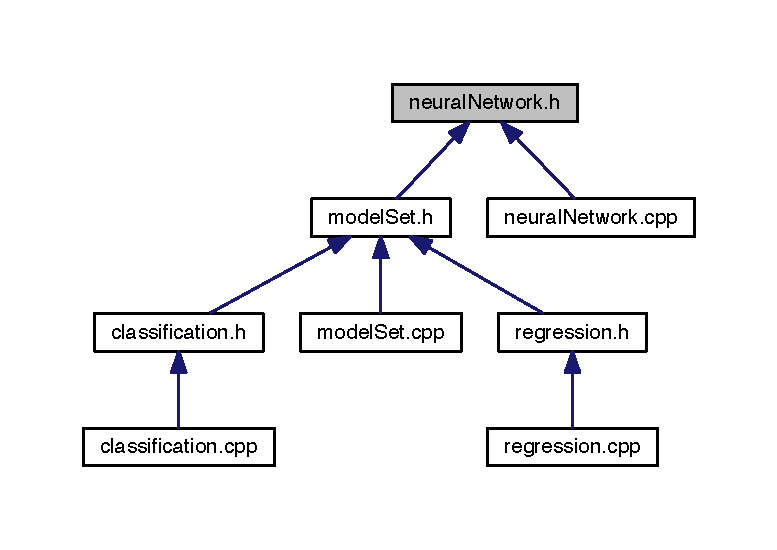
\includegraphics[width=350pt]{neural_network_8h__dep__incl}
\end{center}
\end{figure}
\subsection*{Classes}
\begin{DoxyCompactItemize}
\item 
class \hyperlink{classneural_network}{neural\+Network}
\end{DoxyCompactItemize}
\subsection*{Macros}
\begin{DoxyCompactItemize}
\item 
\#define \hyperlink{neural_network_8h_ac9d3b34ee7e35eab6a81ed21f18f6e64}{L\+E\+A\+R\+N\+I\+N\+G\+\_\+\+R\+A\+TE}~0.\+3
\item 
\#define \hyperlink{neural_network_8h_ab86cb6f507edc7b439a6fb895ab14cc1}{M\+O\+M\+E\+N\+T\+UM}~0.\+2
\item 
\#define \hyperlink{neural_network_8h_ada2f6c75cc0154e34ea6a22ec4aeb665}{N\+U\+M\+\_\+\+E\+P\+O\+C\+HS}~500
\end{DoxyCompactItemize}


\subsection{Macro Definition Documentation}
\mbox{\Hypertarget{neural_network_8h_ac9d3b34ee7e35eab6a81ed21f18f6e64}\label{neural_network_8h_ac9d3b34ee7e35eab6a81ed21f18f6e64}} 
\index{neural\+Network.\+h@{neural\+Network.\+h}!L\+E\+A\+R\+N\+I\+N\+G\+\_\+\+R\+A\+TE@{L\+E\+A\+R\+N\+I\+N\+G\+\_\+\+R\+A\+TE}}
\index{L\+E\+A\+R\+N\+I\+N\+G\+\_\+\+R\+A\+TE@{L\+E\+A\+R\+N\+I\+N\+G\+\_\+\+R\+A\+TE}!neural\+Network.\+h@{neural\+Network.\+h}}
\subsubsection{\texorpdfstring{L\+E\+A\+R\+N\+I\+N\+G\+\_\+\+R\+A\+TE}{LEARNING\_RATE}}
{\footnotesize\ttfamily \#define L\+E\+A\+R\+N\+I\+N\+G\+\_\+\+R\+A\+TE~0.\+3}

\mbox{\Hypertarget{neural_network_8h_ab86cb6f507edc7b439a6fb895ab14cc1}\label{neural_network_8h_ab86cb6f507edc7b439a6fb895ab14cc1}} 
\index{neural\+Network.\+h@{neural\+Network.\+h}!M\+O\+M\+E\+N\+T\+UM@{M\+O\+M\+E\+N\+T\+UM}}
\index{M\+O\+M\+E\+N\+T\+UM@{M\+O\+M\+E\+N\+T\+UM}!neural\+Network.\+h@{neural\+Network.\+h}}
\subsubsection{\texorpdfstring{M\+O\+M\+E\+N\+T\+UM}{MOMENTUM}}
{\footnotesize\ttfamily \#define M\+O\+M\+E\+N\+T\+UM~0.\+2}

\mbox{\Hypertarget{neural_network_8h_ada2f6c75cc0154e34ea6a22ec4aeb665}\label{neural_network_8h_ada2f6c75cc0154e34ea6a22ec4aeb665}} 
\index{neural\+Network.\+h@{neural\+Network.\+h}!N\+U\+M\+\_\+\+E\+P\+O\+C\+HS@{N\+U\+M\+\_\+\+E\+P\+O\+C\+HS}}
\index{N\+U\+M\+\_\+\+E\+P\+O\+C\+HS@{N\+U\+M\+\_\+\+E\+P\+O\+C\+HS}!neural\+Network.\+h@{neural\+Network.\+h}}
\subsubsection{\texorpdfstring{N\+U\+M\+\_\+\+E\+P\+O\+C\+HS}{NUM\_EPOCHS}}
{\footnotesize\ttfamily \#define N\+U\+M\+\_\+\+E\+P\+O\+C\+HS~500}


\hypertarget{nn_embindings_8h}{}\section{nn\+Embindings.\+h File Reference}
\label{nn_embindings_8h}\index{nn\+Embindings.\+h@{nn\+Embindings.\+h}}
{\ttfamily \#include $<$vector$>$}\newline
{\ttfamily \#include $<$emscripten.\+h$>$}\newline
{\ttfamily \#include $<$bind.\+h$>$}\newline
Include dependency graph for nn\+Embindings.\+h\+:\nopagebreak
\begin{figure}[H]
\begin{center}
\leavevmode
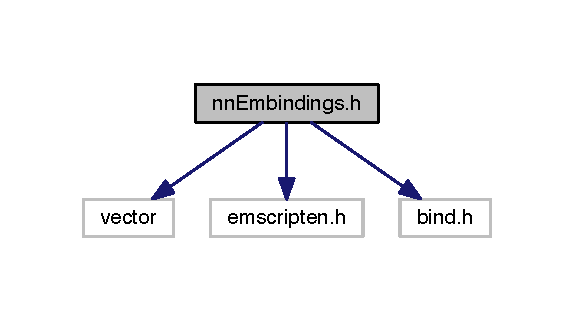
\includegraphics[width=275pt]{nn_embindings_8h__incl}
\end{center}
\end{figure}
\subsection*{Functions}
\begin{DoxyCompactItemize}
\item 
\hyperlink{nn_embindings_8h_a56864121f49285a8b76ba12f64a4c9a4}{E\+M\+S\+C\+R\+I\+P\+T\+E\+N\+\_\+\+B\+I\+N\+D\+I\+N\+GS} (nn\+\_\+module)
\end{DoxyCompactItemize}


\subsection{Function Documentation}
\mbox{\Hypertarget{nn_embindings_8h_a56864121f49285a8b76ba12f64a4c9a4}\label{nn_embindings_8h_a56864121f49285a8b76ba12f64a4c9a4}} 
\index{nn\+Embindings.\+h@{nn\+Embindings.\+h}!E\+M\+S\+C\+R\+I\+P\+T\+E\+N\+\_\+\+B\+I\+N\+D\+I\+N\+GS@{E\+M\+S\+C\+R\+I\+P\+T\+E\+N\+\_\+\+B\+I\+N\+D\+I\+N\+GS}}
\index{E\+M\+S\+C\+R\+I\+P\+T\+E\+N\+\_\+\+B\+I\+N\+D\+I\+N\+GS@{E\+M\+S\+C\+R\+I\+P\+T\+E\+N\+\_\+\+B\+I\+N\+D\+I\+N\+GS}!nn\+Embindings.\+h@{nn\+Embindings.\+h}}
\subsubsection{\texorpdfstring{E\+M\+S\+C\+R\+I\+P\+T\+E\+N\+\_\+\+B\+I\+N\+D\+I\+N\+G\+S()}{EMSCRIPTEN\_BINDINGS()}}
{\footnotesize\ttfamily E\+M\+S\+C\+R\+I\+P\+T\+E\+N\+\_\+\+B\+I\+N\+D\+I\+N\+GS (\begin{DoxyParamCaption}\item[{nn\+\_\+module}]{ }\end{DoxyParamCaption})}


\hypertarget{regression_8cpp}{}\section{regression.\+cpp File Reference}
\label{regression_8cpp}\index{regression.\+cpp@{regression.\+cpp}}
{\ttfamily \#include $<$vector$>$}\newline
{\ttfamily \#include \char`\"{}regression.\+h\char`\"{}}\newline
Include dependency graph for regression.\+cpp\+:\nopagebreak
\begin{figure}[H]
\begin{center}
\leavevmode
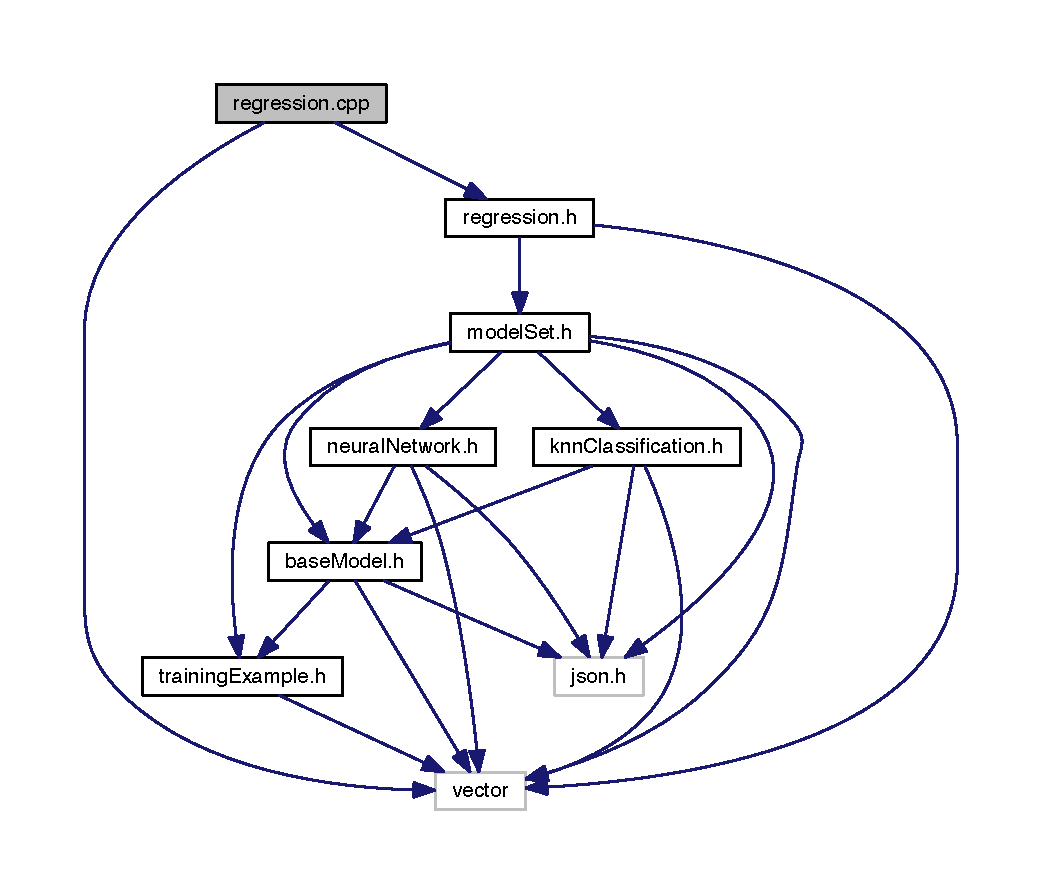
\includegraphics[width=350pt]{regression_8cpp__incl}
\end{center}
\end{figure}

\hypertarget{regression_8h}{}\section{regression.\+h File Reference}
\label{regression_8h}\index{regression.\+h@{regression.\+h}}
{\ttfamily \#include $<$vector$>$}\newline
{\ttfamily \#include \char`\"{}model\+Set.\+h\char`\"{}}\newline
Include dependency graph for regression.\+h\+:\nopagebreak
\begin{figure}[H]
\begin{center}
\leavevmode
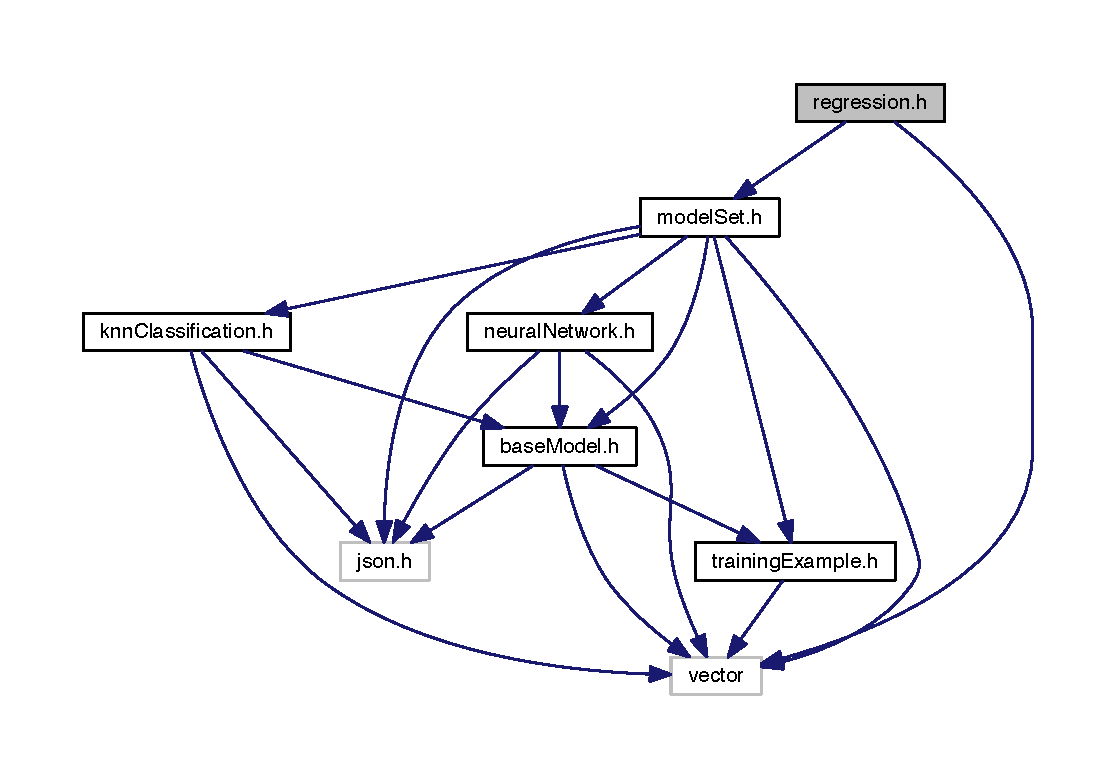
\includegraphics[width=350pt]{regression_8h__incl}
\end{center}
\end{figure}
This graph shows which files directly or indirectly include this file\+:\nopagebreak
\begin{figure}[H]
\begin{center}
\leavevmode
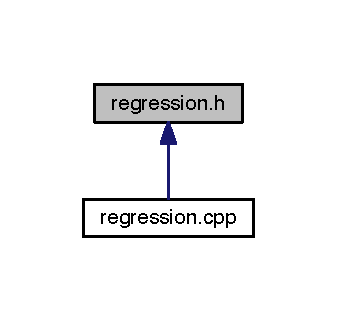
\includegraphics[width=162pt]{regression_8h__dep__incl}
\end{center}
\end{figure}
\subsection*{Classes}
\begin{DoxyCompactItemize}
\item 
class \hyperlink{classregression}{regression}
\end{DoxyCompactItemize}

\hypertarget{regression_embindings_8h}{}\section{regression\+Embindings.\+h File Reference}
\label{regression_embindings_8h}\index{regression\+Embindings.\+h@{regression\+Embindings.\+h}}
{\ttfamily \#include $<$emscripten.\+h$>$}\newline
{\ttfamily \#include $<$bind.\+h$>$}\newline
Include dependency graph for regression\+Embindings.\+h\+:\nopagebreak
\begin{figure}[H]
\begin{center}
\leavevmode
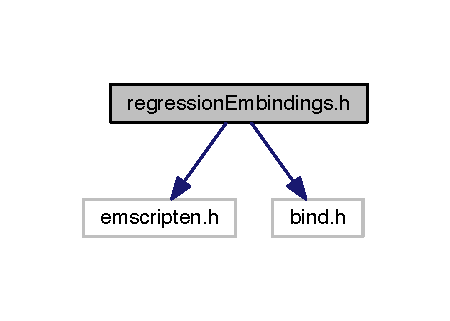
\includegraphics[width=216pt]{regression_embindings_8h__incl}
\end{center}
\end{figure}
\subsection*{Functions}
\begin{DoxyCompactItemize}
\item 
\hyperlink{regression_embindings_8h_a0f2c8f2df64b82cfe84d8974e0dbb277}{E\+M\+S\+C\+R\+I\+P\+T\+E\+N\+\_\+\+B\+I\+N\+D\+I\+N\+GS} (regression\+\_\+module)
\end{DoxyCompactItemize}


\subsection{Function Documentation}
\mbox{\Hypertarget{regression_embindings_8h_a0f2c8f2df64b82cfe84d8974e0dbb277}\label{regression_embindings_8h_a0f2c8f2df64b82cfe84d8974e0dbb277}} 
\index{regression\+Embindings.\+h@{regression\+Embindings.\+h}!E\+M\+S\+C\+R\+I\+P\+T\+E\+N\+\_\+\+B\+I\+N\+D\+I\+N\+GS@{E\+M\+S\+C\+R\+I\+P\+T\+E\+N\+\_\+\+B\+I\+N\+D\+I\+N\+GS}}
\index{E\+M\+S\+C\+R\+I\+P\+T\+E\+N\+\_\+\+B\+I\+N\+D\+I\+N\+GS@{E\+M\+S\+C\+R\+I\+P\+T\+E\+N\+\_\+\+B\+I\+N\+D\+I\+N\+GS}!regression\+Embindings.\+h@{regression\+Embindings.\+h}}
\subsubsection{\texorpdfstring{E\+M\+S\+C\+R\+I\+P\+T\+E\+N\+\_\+\+B\+I\+N\+D\+I\+N\+G\+S()}{EMSCRIPTEN\_BINDINGS()}}
{\footnotesize\ttfamily E\+M\+S\+C\+R\+I\+P\+T\+E\+N\+\_\+\+B\+I\+N\+D\+I\+N\+GS (\begin{DoxyParamCaption}\item[{regression\+\_\+module}]{ }\end{DoxyParamCaption})}


\hypertarget{training_example_8h}{}\section{training\+Example.\+h File Reference}
\label{training_example_8h}\index{training\+Example.\+h@{training\+Example.\+h}}
{\ttfamily \#include $<$vector$>$}\newline
Include dependency graph for training\+Example.\+h\+:\nopagebreak
\begin{figure}[H]
\begin{center}
\leavevmode
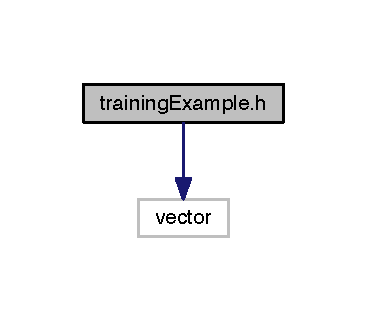
\includegraphics[width=176pt]{training_example_8h__incl}
\end{center}
\end{figure}
This graph shows which files directly or indirectly include this file\+:\nopagebreak
\begin{figure}[H]
\begin{center}
\leavevmode
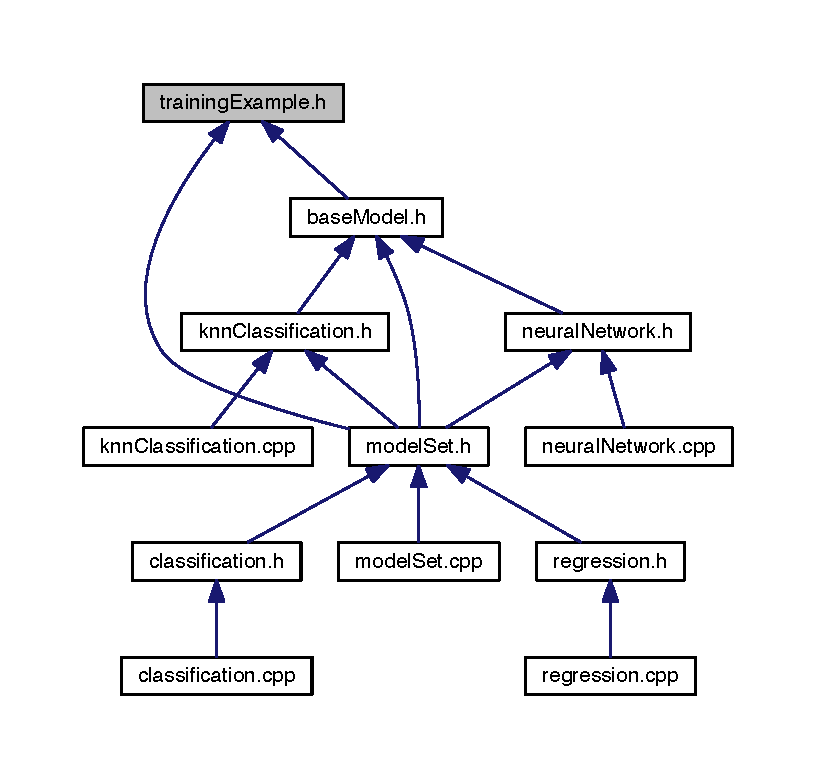
\includegraphics[width=350pt]{training_example_8h__dep__incl}
\end{center}
\end{figure}
\subsection*{Classes}
\begin{DoxyCompactItemize}
\item 
struct \hyperlink{structtraining_example}{training\+Example}
\end{DoxyCompactItemize}

\hypertarget{training_example_embindings_8h}{}\section{training\+Example\+Embindings.\+h File Reference}
\label{training_example_embindings_8h}\index{training\+Example\+Embindings.\+h@{training\+Example\+Embindings.\+h}}
{\ttfamily \#include $<$vector$>$}\newline
{\ttfamily \#include $<$emscripten.\+h$>$}\newline
{\ttfamily \#include $<$bind.\+h$>$}\newline
Include dependency graph for training\+Example\+Embindings.\+h\+:\nopagebreak
\begin{figure}[H]
\begin{center}
\leavevmode
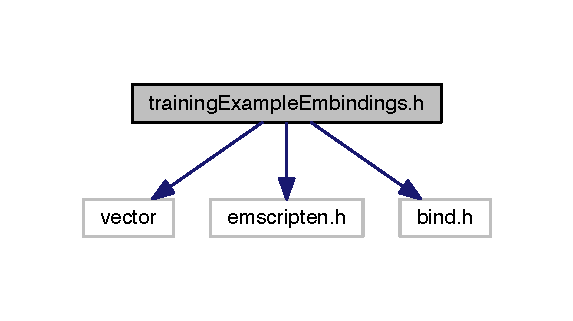
\includegraphics[width=275pt]{training_example_embindings_8h__incl}
\end{center}
\end{figure}
\subsection*{Functions}
\begin{DoxyCompactItemize}
\item 
\hyperlink{training_example_embindings_8h_acea9cc23407d20afe27e8fa64adc4c20}{E\+M\+S\+C\+R\+I\+P\+T\+E\+N\+\_\+\+B\+I\+N\+D\+I\+N\+GS} (stl\+\_\+wrappers)
\end{DoxyCompactItemize}


\subsection{Function Documentation}
\mbox{\Hypertarget{training_example_embindings_8h_acea9cc23407d20afe27e8fa64adc4c20}\label{training_example_embindings_8h_acea9cc23407d20afe27e8fa64adc4c20}} 
\index{training\+Example\+Embindings.\+h@{training\+Example\+Embindings.\+h}!E\+M\+S\+C\+R\+I\+P\+T\+E\+N\+\_\+\+B\+I\+N\+D\+I\+N\+GS@{E\+M\+S\+C\+R\+I\+P\+T\+E\+N\+\_\+\+B\+I\+N\+D\+I\+N\+GS}}
\index{E\+M\+S\+C\+R\+I\+P\+T\+E\+N\+\_\+\+B\+I\+N\+D\+I\+N\+GS@{E\+M\+S\+C\+R\+I\+P\+T\+E\+N\+\_\+\+B\+I\+N\+D\+I\+N\+GS}!training\+Example\+Embindings.\+h@{training\+Example\+Embindings.\+h}}
\subsubsection{\texorpdfstring{E\+M\+S\+C\+R\+I\+P\+T\+E\+N\+\_\+\+B\+I\+N\+D\+I\+N\+G\+S()}{EMSCRIPTEN\_BINDINGS()}}
{\footnotesize\ttfamily E\+M\+S\+C\+R\+I\+P\+T\+E\+N\+\_\+\+B\+I\+N\+D\+I\+N\+GS (\begin{DoxyParamCaption}\item[{stl\+\_\+wrappers}]{ }\end{DoxyParamCaption})}


%--- End generated contents ---

% Index
\backmatter
\newpage
\phantomsection
\clearemptydoublepage
\addcontentsline{toc}{chapter}{Index}
\printindex

\end{document}
